% SPDX-License-Identifier: CC-BY-SA-4.0
%
% Copyright (c) 2020 Philipp Le
%
% Except where otherwise noted, this work is licensed under a
% Creative Commons Attribution-ShareAlike 4.0 License.
%
% Please find the full copy of the licence at:
% https://creativecommons.org/licenses/by-sa/4.0/legalcode

\chapter{Time-Continuous Signals and Systems}

\begin{refsection}

All signals considered in this chapter are \index{signal!deterministic signal} \textbf{deterministic}, i.e., its values are predictable at any time. Especially, the values can be calculated by a mathematical equation. In contrast, \emph{random} signals are not predictable. Its values are subject to a random process, which must be modelled stochastically.

Furthermore, the signals considered here are time-continuous.

\index{signal!time-continuous}
\begin{figure}[H]
	\centering
	\begin{tikzpicture}
		\draw node[block](Signals){\textbf{Signal}\\ \textbf{(deterministic)}};
		\draw node[block, below left=of Signals](Periodic){Periodic};
		\draw node[block, below right=of Signals](NonPeriodic){Non-periodic};
		\draw node[block, below left=of Periodic](Mono){Mono-chromatic};
		\draw node[block, below right=of Periodic](Multi){Multi-frequent};
		
		\draw [-latex] (Signals) -- (Periodic);
		\draw [-latex] (Signals) -- (NonPeriodic);
		\draw [-latex] (Periodic) -- (Mono);
		\draw [-latex] (Periodic) -- (Multi);
	\end{tikzpicture}
	\caption{Classification of signals}
	\label{fig:ch02:timecont_signals_classif}
\end{figure}

\section{Mono-Chromatic Signals}

\subsection{Real-Valued Signals and Phasor}

\paragraph{Representation by A Real-Valued Function.}

The mono-chromatic signal $x_{mc}(t)$ is defined by:
\begin{equation}
	x_{mc}(t) = \hat{X} \cdot \cos\left(\omega_0 t - \varphi_0\right)
	\label{eq:ch02:mono_chrom_eq}
\end{equation}%
\nomenclature[Sx]{$x_{mc}(t)$, $\underline{x}_{mc}(t)$}{Mono-chromatic signal}%
where

\begin{tabular}{ll}
	$\hat{X}$ & is the \index{amplitude} \textbf{amplitude} of the signal \nomenclature[Sx]{$\hat{X}$}{Amplitude of a mono-chromatic signal}, \\
	$\omega_0$ & is the \index{angular frequency} \textbf{angular frequency} of the signal \nomenclature[So]{$\omega_0$}{Angular frequency of a mono-chromatic signal}, \\
	$\varphi_0$ & is the \index{phase} \textbf{phase} of the signal \nomenclature[Sp]{$\varphi_0$}{Phase of a mono-chromatic signal}, \\
	$t \in \mathbb{R}$ & is the real-value time variable and continuously defined \nomenclature[St]{$t$}{Time (continuous)}.
\end{tabular}

In fact, the sine function $\sin()$ is mono-chromatic, too. However, it can be derived from \eqref{eq:ch02:mono_chrom_eq} with $\varphi_0 = \SI{90}{\degree}$.

\begin{equation*}
	x_{sin}(t) = \hat{X} \cdot \sin\left(\omega_0 t\right) = \cos\left(\omega_0 t - \SI{90}{\degree}\right)
\end{equation*}

The angular frequency is connected to the \index{frequency} \textbf{frequency}.
\begin{equation}
	\omega_0 = 2 \pi f_0
\end{equation}%
\nomenclature[Sf]{$f_0$}{Frequency of a mono-chromatic signal}

\begin{attention}
	You must not confuse the terms \emph{frequency} and \emph{angular frequency}!
\end{attention}

The inverse of the frequency is the \index{period} \textbf{period} $T_0$. It is the time interval at which the signal repeats.
\begin{equation}
	T_0 = \frac{1}{f_0} = \frac{2 \pi}{\omega_0}
\end{equation}%
\nomenclature[St]{$T_0$}{Period of a mono-chromatic signal}

Be aware of the units. The period $T_0$ is defined in seconds \si{s}. The frequency $f_0$ is the inverse of seconds, which is Hertz \si{Hz}. The angular frequency $\omega_0$ is the inverse of seconds, too. However, it is never given in Hertz, only in \si{rad/s} or, more commonly, \si{1/s}.

\begin{table}[H]
	\centering
	\caption{Units}
	\begin{tabular}{|l|l|}
		\hline
		Period $T_0$ & \si{s} \\
		\hline
		Frequency $f_0$ & \si{Hz} \\
		\hline
		Angular frequency $\omega_0$ & \si{1/s} \; (never Hertz!) \\
		\hline
	\end{tabular}
\end{table}

The actual unit of the signal is derived from its amplitude $\hat{X}$ which can be any physical measure.

\paragraph{Representation by A Complex-Valued Phasor.}

A graphical view on the creation of a cosine signal is depicted in Figure \ref{fig:ch02:cos_creation}.

\begin{figure}[H]
	\centering
	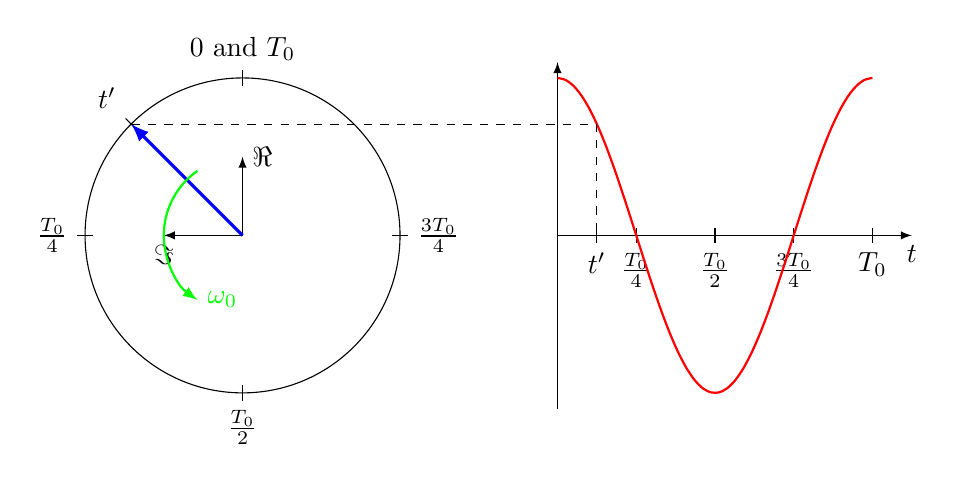
\begin{tikzpicture}
		\begin{scope}[shift={(0, 0)}]
			\draw[-latex] (0,0) -- (4.5,0) node[below, align=left]{$t$};
			\draw[-latex] (0,-2.2) -- (0,2.2);
			\draw (1,0.1) -- (1,-0.1) node[below, align=center]{$\frac{T_0}{4}$};
			\draw (2,0.1) -- (2,-0.1) node[below, align=center]{$\frac{T_0}{2}$};
			\draw (3,0.1) -- (3,-0.1) node[below, align=center]{$\frac{3 T_0}{4}$};
			\draw (4,0.1) -- (4,-0.1) node[below, align=center]{$T_0$};
			
			\draw (0.5,0.1) -- (0.5,-0.1) node[below, align=center]{$t'$};
			
			\draw[red, thick, smooth, domain=0:4, samples=40] plot (\x, {2*cos( 360 * \x / 4 )});
		\end{scope}
		\begin{scope}[shift={(-4, 0)}]
			\draw[draw] (0:2) arc(0:360:2);
			\draw[-latex] (0,0) -- (0,1) node[right, align=left]{$\Re$};
			\draw[-latex] (0,0) -- (-1,0) node[below, align=center]{$\Im$};
			
			\draw (180:1.9) -- (180:2.1) node[left, align=center]{$\frac{T_0}{4}$};
			\draw (270:1.9) -- (270:2.1) node[below, align=center]{$\frac{T_0}{2}$};
			\draw (0:1.9) -- (0:2.1) node[right, align=center]{$\frac{3 T_0}{4}$};
			\draw (90:1.9) -- (90:2.1) node[above, align=center]{$0$ and $T_0$};
			
			\draw (135:1.9) -- (135:2.1) node[above left, align=right]{$t'$};
			
			\draw[very thick, blue, -latex] (135:0) -- (135:2);
			
			
			\draw[thick, green, -latex] (125:1) arc(125:235:1) node[right, align=left]{$\omega_0$};
		\end{scope}
		
		\draw[dashed] (-5.414, 1.414) -- (0.5, 1.414) -- (0.5, 0);
	\end{tikzpicture}
	\caption[Generation of a sinusoidal shape]{Generation of a sinusoidal shape. Imagine, there is a pointer (blue) with one side fixed to a point. Now, it begins rotating counter-clockwise with an angular frequency of $\omega_0$ (green). The arrow of the pointer draws a circle (left side). Each angle of the pointer is related to a time instance. The blue pointer is the current position at time instance $t'$. Its vertical value is projected into the time plot, forming the cosine wave (red).}
	\label{fig:ch02:cos_creation}
\end{figure}

You may now some relations:
\begin{itemize}
	\item A full rotation of the pointer takes exactly one period $T_0$.
	\item The orange cosine curve can be horizontally shifted by redefining the original angle of the pointer at $T_0$. This offset angle is the phase $\varphi_0$.
	\item The length of the pointer and the radius of the circle is the amplitude $\hat{X}$.
\end{itemize}

A mono-chromatic signal can be described by its three parameters
\begin{itemize}
	\item Amplitude $\hat{X}$
	\item Phase $\varphi_0$
	\item Frequency $\omega_0$
\end{itemize}

When a signal passes through a \ac{LTI} system, the amplitude, the phase or both may change. However, the frequency never changes. Thus, the frequency $\omega_0$ is assumed to be constant and neglected. Consequently, the parameters
\begin{itemize}
	\item amplitude $\hat{X}$ and
	\item phase $\varphi_0$
\end{itemize}
remain. Both are absorbed by the complex-valued \index{phasor} \textbf{phasor} $\underline{X}$, which uniquely describes a mono-chromatic signal.
\begin{equation}
	\underline{X} = \hat{X} \cdot e^{-j \varphi_0} = \hat{X} \angle -\varphi_0
\end{equation}%
\nomenclature[Np]{$r \angle \varphi$}{Complex with absolute value $r$ and phase $\varphi$ (e.g. phasor) in angle notation}

\begin{excursus}{Complex numbers}
	$j$ is the \index{imaginary unit} \textbf{imaginary unit}. It satisfies the equation
	\begin{equation}
		j^2 = -1
	\end{equation}%
	\nomenclature[Sj]{$j$}{Imaginary unit}%
	There is no real number $j \notin \mathbb{R}$ which satisfies the above solution. $j$ spans the set of complex numbers $\mathbb{C}$.
	
	In mathematics, the imaginary unit is noted as $i$. In engineering context, $j$ is used instead, because $i$ is the symbol of the electric current.
	
	A complex number $\underline{c} \in \mathbb{C}$ can be noted in \index{cartesian form} \textbf{cartesian form}:
	\begin{equation}
		\underline{c} = a + j b
	\end{equation}
	$a \in \mathbb{R}$ is the \index{real part} \textbf{real part} of $\underline{c}$. $b \in \mathbb{R}$ is the \index{imaginary part} \textbf{imaginary part} $\underline{c}$.
	\begin{subequations}
		\begin{align}
			a &= \Re\{\underline{c}\} \\
			b &= \Im\{\underline{c}\}
		\end{align}
	\end{subequations}%
	\nomenclature[Fr]{$\Re\{\underline{c}\}$}{Extracting the real part of the complex number $\underline{c}$}%
	\nomenclature[Fi]{$\Im\{\underline{c}\}$}{Extracting the imaginary part of the complex number $\underline{c}$}%
	Complex numbers $\underline{c}$ always carry an underline in this lecture to distinguish them from real numbers. However, this is not mandatory.

	Another notation is the \index{polar form} \textbf{polar form}:
	\begin{equation}
		\underline{c} = r \cdot e^{j \varphi}
	\end{equation}
	with
	\begin{subequations}
		\begin{align}
			r &= |\underline{c}| = \sqrt{\Re\{\underline{c}\}^2 + \Im\{\underline{c}\}^2} \\
			\varphi &= \mathrm{atan2} \left(\Im\{\underline{c}\}, \Re\{\underline{c}\}\right) \\
			e^{j \varphi} &= \cos \varphi + j \sin \varphi
		\end{align}
	\end{subequations}
	The polar form can be written in \index{angle notation} \textbf{angle notation}:
	\begin{equation}
		\underline{c} = r \angle \varphi
	\end{equation}
	$r \in \mathbb{R}$ and $\varphi \in \mathbb{R}$ are the \index{polar coordinates} \textbf{polar coordinates}.
\end{excursus}

The phasor $\underline{X} \in \mathbb{C}$ is a complex number, which is mostly represented in polar coordinates (see Figure \ref{fig:ch02:cmplxplane_phasor}).

\begin{figure}[H]
	\centering
	\begin{tikzpicture}
	\draw[->] (-3.2,0) -- (3.2,0) node[below, align=left]{$\Re$};
	\draw[->] (0,-3.2) -- (0,3.2) node[left, align=right]{$\Im$};
	\draw[->, thick] (0, 0) -- (-40:3) node[right, align=left]{Complex phasor $\underline{X}$\\ (position at $t = 0$)};
	\draw (0:1.5) arc(0:-40:1.5) node[midway, right, align=left]{Phase $\varphi_0$};
	
	\draw[->, dashed] (-50:1) arc(-50:30:1) node[right, align=left]{$\omega_0$};
	\end{tikzpicture}
	\caption{Phasor in the complex plane}
	\label{fig:ch02:cmplxplane_phasor}
\end{figure}

Figure \ref{fig:ch02:cmplxplane_phasor} depicts the phasor in the complex plane. Figure \ref{fig:ch02:cos_creation} shows a complex plane, too. Please note that both complex planes are rotated by \SI{90}{\degree} with respect to each other.

\begin{fact}
	The phasor of a signal is a signal parameter, constant and \underline{not} time-dependent.
\end{fact}

The current position of the pointer $\underline{x}(t)$ in the complex plane is obtained by rotating it. It makes a full rotation each $T_0$ periods. Therefore, it rotates at an angular frequency of $\omega_0$. The rotation is a multiplication by $e^{j \omega_0 t}$ in the complex plane. $\underline{x}(t) \in \mathbb{C}$ is a complex value, too.
\begin{equation}
	\underline{x_{mc}}(t) = \underline{X} \cdot e^{j \omega_0 t} = \hat{X} \cdot e^{-j \varphi_0} \cdot e^{j \omega_0 t}
\end{equation}

The real-valued function can be obtained by extracting the real part of the complex-valued current value.
\begin{equation}
	x_{mc}(t) = \Re\left\{\underline{x_{mc}}(t)\right\}
\end{equation}

\begin{proof}{}
	\begin{equation}
		\begin{split}
			x_{mc}(t) &= \Re\left\{\underline{x_{mc}}(t)\right\} \\
			 &= \Re\left\{\hat{X} \cdot e^{-j \varphi_0} \cdot e^{j \omega_0 t}\right\} \\
			 &= \hat{X} \cdot \Re\left\{e^{j \left(\omega_0 t - \varphi_0\right)}\right\} \\
			 &= \hat{X} \cdot \Re\left\{\cos \left(\omega_0 t - \varphi_0\right) + j \sin \left(\omega_0 t - \varphi_0\right)\right\} \\
			 &= \hat{X} \cdot \cos \left(\omega_0 t - \varphi_0\right) \\
		\end{split}
	\end{equation}
\end{proof}

\subsection{Complex-Valued Signals}

\begin{excursus}{Are there complex-valued, mono-chromatic signals?}
	Yes, there is.
	\begin{equation}
		\underline{x}_{mc,e}(t) = \hat{X} \cdot e^{j \left(\omega_0 t - \varphi_0\right)}
	\end{equation}
	is a complex-valued, mono-chromatic signal. We will come back to it later, but not in this chapter.
	
	\vspace{0.5em}
	Phasor representation:
	\begin{equation}
		\underline{x}_{mc,e}(t) = \underline{X} \cdot e^{- j \omega_0 t}
	\end{equation}
	With the phasor $\underline{X}$:
	\begin{equation}
		\underline{X} = \hat{X} \cdot e^{- j \varphi_0} =  \hat{X} \angle -\varphi_0
	\end{equation}
	If you use a phasor, it must be clear from the context, whether you refer to a real-valued or complex-valued, mono-chromatic signal.
\end{excursus}

\section{Periodic Signals and Fourier Series}

Periodic signals $x_p(t)$ comprises a class of signals which indefinitely repeat at constant time intervals $T_0$.
\begin{equation}
	x_p(t + n T_0) = x_p(t) \qquad \forall \; n \in \mathbb{Z}, \quad \mathbb{Z} = \left\{..., -2, -1, 0, 1, 2, ...\right\}
\end{equation}%
\nomenclature[Sx]{$x_p(t)$, $\underline{x}_p(t)$}{Periodic signal}%
\nomenclature[Sn]{$n$}{Integer enumerator}

Mono-chromatic signals are a special kind of periodic signals. Multi-frequent signals are composed a limited or unlimited number of mono-chromatic signals, which superimpose. Multi-frequent signals are periodic signals in general.

\begin{fact}
	Each periodic signal can be decomposed into a superposition of mono-chromatic signals.
\end{fact}

The inverse of the period $T_0$ is $f_0$, which is the \textbf{base frequency}. This is the frequency at the periodic pattern repeats. Again, frequency and angular frequency $\omega_0 = 2 \pi f_0$ must be distinguished.

The periodic signal can now be decomposed in cosine and sine functions with integer multiples of the base frequency $f_0$ or base angular frequency $\omega_0$, respectively. They are called \index{harmonics} \textbf{harmonics}.
\begin{equation}
	\begin{split}
		x_p(t) &= \sum\limits_{n=0}^{\infty} a_n \cos\left(n \omega_0 t\right) + \sum\limits_{m=0}^{\infty} b_m \sin\left(m \omega_0 t\right) \qquad \forall \; n, m \in \mathbb{N} = \left\{0, 1, 2, ...\right\} \\
		 &= a_0 + \sum\limits_{n=1}^{\infty} a_n \cos\left(n \omega_0 t\right) + \sum\limits_{m=1}^{\infty} b_m \sin\left(m \omega_0 t\right) \\
	\end{split}
	\label{eq:ch02:fourier_series}
\end{equation}

What happened to $n = 0$ and $m = 0$? $\cos(0) = 1$ and $\sin(0) = 0$. That's it.

Comparing to the mono-chromatic signals, what happened to the phase $\varphi_0$? The phase $\varphi_0$ is a characteristic of mono-chromatic signals. It is completely absorbed by the coefficients $a_n$ and $b_n$ of the cosine and sine functions.

\subsection{Orthogonality}
\index{orthogonality}
The cosine and sine functions are orthogonal to each other. In geometry, two vectors $\vect{a}$ and $\vect{b}$ are orthogonal, if the angle between them is \SI{90}{\degree}. In this case, their inner product is zero.
\begin{equation}
	\langle \vect{a}, \vect{b} \rangle = 0
\end{equation}%
\nomenclature[Fa]{$\langle \vect{a}, \vect{b} \rangle$}{Inner product}

More generally, two functions $f(x)$ and $g(x)$ are orthogonal if their \index{inner product} \textbf{inner product} $\langle f, g \rangle$ is zero. 
\begin{equation}
	0 \stackrel{!}{=} \langle f, g \rangle_w = \int\limits_{a}^{b} f(x) g(x) w(x) \, \mathrm{d} x
\end{equation}
$w(x)$ is a non-negative weight function, which is $w(x) = 1$ in simple cases like this one.

Now, you can prove that the cosine and sine functions are orthogonal to each other.
\begin{equation}
	\int\limits_{-\frac{T_0}{2}}^{\frac{T_0}{2}} \cos\left(n \omega_0 t\right) \sin\left(m \omega_0 t\right) \, \mathrm{d} t = 0 \qquad \forall \; n, m \in \mathbb{Z}
	\label{eq:ch02:orth_rel_cos_sin}
\end{equation}

Furthermore, the sine and cosine functions with \underline{different} indices are orthogonal to each other.
\begin{equation}
	\int\limits_{-\frac{T_0}{2}}^{\frac{T_0}{2}} \cos\left(n \omega_0 t\right) \cos\left(p \omega_0 t\right) \, \mathrm{d} t = \frac{\pi}{\omega_0} \cdot \delta_{np} \qquad \forall \; n, p \in \mathbb{N} \backslash \{0\}
	\label{eq:ch02:orth_rel_cos}
\end{equation}
\begin{equation}
	\int\limits_{-\frac{T_0}{2}}^{\frac{T_0}{2}} \sin\left(m \omega_0 t\right) \sin\left(q \omega_0 t\right) \, \mathrm{d} t = \frac{\pi}{\omega_0} \cdot \delta_{mq} \qquad \forall \; m, q \in \mathbb{N} \backslash \{0\}
	\label{eq:ch02:orth_rel_sin}
\end{equation}
with the Kronecker delta
\begin{equation}
	\delta_{uv} = \begin{cases}
		1 & \qquad \text{if } u = v, \\
		0 & \qquad \text{if } u \neq v
	\end{cases}
	\label{eq:ch02:kronecker_delta}
\end{equation}%
\nomenclature[Fd]{$\delta_{uv}$}{Kronecker delta}

The \index{orthogonality relations} \textbf{orthogonality relations} \eqref{eq:ch02:orth_rel_cos_sin}, \eqref{eq:ch02:orth_rel_cos} and \eqref{eq:ch02:orth_rel_sin} point out:
\begin{itemize}
	\item Cosine functions are orthogonal if their indices are different. I.e., $n \neq p$ in \eqref{eq:ch02:orth_rel_cos}.
	\item Sine functions are orthogonal if their indices are different. I.e., $m \neq q$ in \eqref{eq:ch02:orth_rel_sin}.
	\item Cosine and sine function are orthogonal independent of their indices.
	\item The indices are the integer multiples of the base frequency $\omega_0$ (harmonics).
\end{itemize}

\subsection{Extraction of The Coefficients}

The orthogonality relations are useful to extract the coefficients $a_n$ and $b_n$ in \eqref{eq:ch02:fourier_series}. Given is the input signal $\tilde{x}_p(t)$ whose coefficient shall be determined. Following assumptions can be derived from the properties of a periodic signal:
\begin{itemize}
	\item $\tilde{x}_p(t)$ is composed of mono-chromatic cosine and sine functions.
	\item All cosine and sine functions have integer multiples of the base frequency.
	\item Each cosine and sine function has a different weight -- the coefficient.
\end{itemize}

Using the orthogonality relations, the coefficients $\tilde{a}_n$ and $\tilde{b}_n$ can be obtained by:
\begin{subequations}
	\begin{align}
		\tilde{a}_n &= \frac{\omega_0}{\pi} \int\limits_{-\frac{T_0}{2}}^{\frac{T_0}{2}} \tilde{x}_p(t) \cdot \cos\left(n \omega_0 t\right) \, \mathrm{d} t \label{eq_ch02_fourier_series_coeff_an} \qquad \forall \; n > 0 \\
		\tilde{b}_m &= \frac{\omega_0}{\pi} \int\limits_{-\frac{T_0}{2}}^{\frac{T_0}{2}} \tilde{x}_p(t) \cdot \sin\left(m \omega_0 t\right) \, \mathrm{d} t \label{eq_ch02_fourier_series_coeff_bm} \qquad \forall \; m > 0 \\
		\tilde{a}_0 &= \frac{\omega_0}{2 \pi} \int\limits_{-\frac{T_0}{2}}^{\frac{T_0}{2}} \tilde{x}_p(t) \, \mathrm{d} t \\
		\tilde{b}_0 &= 0
	\end{align}
\end{subequations}
\textit{Remark: } $a_0$ and $b_0$ need a special treatment, because of slightly changed orthogonality relations.

\begin{proof}{Parameter Extraction for $\tilde{a}_n$}
	Given is a periodic function $\tilde{x}_p(t)$, which can be decomposed into:
	\begin{equation}
		\tilde{x}_p(t) = \sum\limits_{p=0}^{\infty} \tilde{a}_p \cos\left(p \omega_0 t\right) + \sum\limits_{q=0}^{\infty} \tilde{b}_q \sin\left(q \omega_0 t\right)
		\label{eq_ch02_proof_per_sig_example}
	\end{equation}
	The coefficient $\tilde{a}_n$ is of interest.
	
	Inserting \eqref{eq_ch02_proof_per_sig_example} into \eqref{eq_ch02_fourier_series_coeff_an}, yields
	\begin{equation}
		\tilde{a}_n = \frac{\omega_0}{\pi} \int\limits_{-\frac{T_0}{2}}^{\frac{T_0}{2}} \left(\sum\limits_{p=0}^{\infty} \tilde{a}_p \cos\left(p \omega_0 t\right) + \sum\limits_{q=0}^{\infty} \tilde{b}_q \sin\left(q \omega_0 t\right)\right) \cdot \cos\left(n \omega_0 t\right) \, \mathrm{d} t
	\end{equation}
	Due to the orthogonality relations, \underline{all products containing a sine function} and \underline{all products containing a cosine function with the index $n \neq p$} become zero. Furthermore, following must be true: $n = p$
	
	\begin{equation}
		\tilde{a}_n = \tilde{a}_p \frac{\omega_0}{\pi} \int\limits_{-\frac{T_0}{2}}^{\frac{T_0}{2}} \cos\left(p \omega_0 t\right) \cdot \cos\left(n \omega_0 t\right) \, \mathrm{d} t \qquad \text{if } \; n = p
	\end{equation}
	
	Using \eqref{eq:ch02:orth_rel_cos}, the integral resolves to:
	\begin{equation}
		\tilde{a}_n = \tilde{a}_p \frac{\omega_0}{\pi} \frac{\pi}{\omega_0} \qquad \text{if } \; n = p
	\end{equation}
	
	In the end, it could be proven that $\tilde{a}_n = \tilde{a}_p$ for $n = p$.
	
	The proof is analogous for the coefficient $b_n$.
\end{proof}

$\cos\left(n \omega_0 t\right)$ can be seen as a ``test function'', which is used to extract the component with the index $n$. The proof points out:
\begin{itemize}
	\item All sine components are erased by $\cos\left(n \omega_0 t\right)$, due to the orthogonality relations.
	\item All cosine function with index $p \neq n$ are erased by $\cos\left(n \omega_0 t\right)$, due to the orthogonality relations.
\end{itemize}
For $b_m$, $\sin\left(m \omega_0 t\right)$ is analogous.

\begin{excursus}{Illustration of The ``Test Function''}
	For illustration of the ``test functions'', image you have a radio and want to hear a specific station. You tune to the frequency on which the station is broadcasting. All other signals are filtered out, you don't want to hear them. Actually, the radio does not employ orthogonality in this case. However, this illustration might help to understand the meaning of $\cos\left(n \omega_0 t\right)$ and $\sin\left(m \omega_0 t\right)$ \underline{in connection} with the orthogonality relations.
\end{excursus}

A special case is the coefficient $\tilde{a}_0$.
\begin{equation}
	\tilde{a}_0 = \frac{\omega_0}{\pi} \int\limits_{-\frac{T_0}{2}}^{\frac{T_0}{2}} \tilde{x}_p(t) \, \mathrm{d} t
\end{equation}
$\cos\left(n \omega_0 t\right)$ is $1$ for $n = 0$. $\tilde{a}_0$ is the \index{DC offset} \textbf{\ac{DC} offset} of the signal. The above formula is known as the calculation of the signal mean in electrical engineering.

\begin{definition}{Fourier series}
	The composition of a series of mono-chromatic signals as shown in \eqref{eq:ch02:fourier_series} is called \index{Fourier series} \textbf{Fourier series}.
	\begin{equation*}
		x_p(t) = \sum\limits_{n=1}^{\infty} a_n \cos\left(n \omega_0 t\right) + \sum\limits_{m=1}^{\infty} b_m \sin\left(m \omega_0 t\right)
	\end{equation*}
	
	The coefficients can be calculated using \eqref{eq_ch02_fourier_series_coeff_an} and \eqref{eq_ch02_fourier_series_coeff_bm}.
\end{definition}

\subsection{Complex-Valued Fourier Series}

A complex-valued, periodic signal $\underline{x_p}(t)$ can be decomposed into complex-valued mono-chromatic signals. The coefficients $\underline{c}_n$ are phasors.
\begin{equation}
	\underline{x_p}(t) = \sum\limits_{n = -\infty}^{\infty} \underline{c}_n \cdot e^{j n \omega_0 t} \qquad \forall \; n \in \mathbb{Z}
	\label{eq:ch02:fourier_series_cmplx}
\end{equation}

The coefficients $\underline{\tilde{c}}_n$ of an input signal $\underline{\tilde{x}_p}(t)$ can be determined by:
\begin{equation}
	\underline{\tilde{c}}_n = \frac{\omega_0}{2 \pi} \int\limits_{-\frac{T_0}{2}}^{\frac{T_0}{2}} \underline{\tilde{x}_p}(t) \cdot e^{-j n \omega_0 t} \, \mathrm{d} t
	\label{eq_ch02_fourier_series_coeff_cn}
\end{equation}

It is based on the orthogonality relation:
\begin{equation}
	\int\limits_{-\frac{T_0}{2}}^{\frac{T_0}{2}} e^{j n \omega_0 t} e^{-j p \omega_0 t} \, \mathrm{d} t = \frac{2 \pi}{\omega_0} \cdot \delta_{np} \qquad \forall \; n, p \in \mathbb{Z}
	\label{eq:ch02:orth_rel_exp}
\end{equation}

\vspace*{1em}

\begin{definition}{Complex-Valued Fourier series}
	A complex-valued, periodic signal $\underline{x_p}(t)$ can be decomposed into a series complex-valued mono-chromatic signals \eqref{eq:ch02:fourier_series_cmplx} -- the \index{Fourier series!complex-valued} \textbf{complex-valued Fourier series}.
	\begin{equation*}
		\underline{x_p}(t) = \sum\limits_{n = -\infty}^{\infty} \underline{c}_n \cdot e^{j n \omega_0 t} \qquad \forall \; n \in \mathbb{Z}
	\end{equation*}
	
	The coefficients can be calculated using \eqref{eq_ch02_fourier_series_coeff_cn}.
\end{definition}

\subsection{Amplitude and Phase Spectra}

Let's consider the complex-valued Fourier series $\underline{x_p}(t)$ \eqref{eq:ch02:fourier_series_cmplx}. The coefficients $\underline{c}_n$ are phasors. Its absolute value (amplitude) $|\underline{c}_n|$ and argument (phase) $\arg\left(\underline{c}_n\right)$ can now be plotted over the index $n$. The index $n \in \mathbb{Z}$ is discrete. Thus, the resulting plots are value-discrete in the dimension of $n$. In contrast, the amplitudes and phases are value-continuous.

\begin{definition}{Spectrum of a period signal}
	\begin{itemize}
		\item The plot of the amplitude $|\underline{c}_n|$ is called \index{amplitude spectrum} \textbf{amplitude spectrum}.
		\item The plot of the phase $\arg\left(\underline{c}_n\right)$ is called \index{phase spectrum} \textbf{phase spectrum}.
		\item When referring to the \index{spectrum} \textbf{spectrum}, generally both amplitude and phase, or their complex-valued representation of $\underline{c}_n$ is meant.
	\end{itemize}
\end{definition}

\begin{fact}
	The index $n \in \mathbb{Z}$ is discrete. The plots of the spectrum are value-discrete in the dimension of $n$.
\end{fact}

When considering a complex-valued signal $\underline{x_p}(t)$, both amplitude and phase can take any value, with following constraints:
\begin{itemize}
	\item The amplitude $|\underline{c}_n|$ is always a positive real number.
	\item The phase $\arg\left(\underline{c}_n\right)$ a real number from the interval $[-\pi, +\pi]$.
\end{itemize}%
\nomenclature[Fa]{$|\cdot|$}{Absolute value of $\cdot$}%
\nomenclature[Fa]{$\arg\left(\cdot\right)$}{Argument (angle) of $\cdot$}

If the signal $\underline{x_p}(t) = x_p(t)$ is real-valued, i.e., $\Im\left\{\underline{c}_n(t)\right\} = 0$, the values of $\underline{c}_n$ are even more constrained by the \index{spectrum!symmetry rules} \textbf{symmetry rules}:
\begin{itemize}
	\item The coefficients $\underline{c}_n \in \mathbb{C}$ are still complex-valued phasors.
	\item But, the coefficients $\underline{c}_n$ show a special symmetry.
	\begin{itemize}
		\item The amplitude spectrum $|\underline{c}_n|$ is an \underline{even function}. It is symmetric with respect to the $y$-axis.
		\item The phase spectrum $\arg\left(\underline{c}_n\right)$ is an \underline{odd function}. It is symmetric with respect to the origin.
		\item As a consequence, the phase of $\arg\left(\underline{c}_0\right)$ at $n = 0$ must be either $0$ or $\pm \pi$. Note that, $+\pi$ is identical to $-\pi$ in the complex plane. The phase is the sign of the \ac{DC} bias: $\arg\left(\underline{c}_0\right) = 0$ means positive \ac{DC} bias and $\arg\left(\underline{c}_0\right) = \pi$ means negative \ac{DC} bias.
	\end{itemize}
\end{itemize}
These symmetry rules apply for \underline{all} real-valued signals $\underline{x_p}(t) = x_p(t) \in \mathbb{R}$. The symmetry rules ensure that the mono-chromatic components of the Fourier series \eqref{eq:ch02:fourier_series_cmplx} sum up to a real value at each time instance $t \in \mathbb{R}$.

\begin{definition}{Hermitian function}
	A complex-valued function $\underline{f}(t)$ is a \index{Hermitian function} \textbf{Hermitian function} if
	\begin{equation}
		\overline{\underline{f}(t)} = \underline{f}(-t)
		\label{eq:ch02:hermitian}
	\end{equation}%
	\nomenclature[Na]{$\overline{\left(\cdot\right)}$}{Complex conjugate of $\left(\cdot\right)$}
	where $\overline{\left(\cdot\right)}$ denotes the complex conjugate.
	
	Hermitian function are \index{conjugate symmetric} \textbf{conjugate symmetric}.
\end{definition}

$\underline{c}_n$ is Hermitian if and only if $\underline{x_p}(t) = x_p(t)$ is real-valued.

The symmetry rules do \underline{not} apply for complex-valued signals $\underline{x_p}(t) \in \mathbb{C}$.

\begin{figure}[H]
	\centering
	\begin{tikzpicture}
		\begin{axis}[
			height={0.25\textheight},
			width=0.6\linewidth,
			scale only axis,
			xlabel={$n$},
			ylabel={$|\underline{c}_n|$},
			%grid style={line width=.6pt, color=lightgray},
			%grid=both,
			grid=none,
			axis lines=left,
			legend pos=north east,
			xmin=-4,
			xmax=4,
			ymin=0,
			ymax=3,
			xtick={-3, -2, ..., 3},
			ytick={0, 0.5, ..., 2.5},
			axis y line=middle,
			axis x line=middle,
			every axis x label/.style={
				at={(ticklabel* cs:1.05)},
				anchor=north,
			},
			every axis y label/.style={
				at={(ticklabel* cs:1.05)},
				anchor=east,
			}
		]
			\addplot[red, thick] coordinates {(-3, 0) (-3, 2.0)};
			\addplot[red, thick] coordinates {(-2, 0) (-2, 0.4)};
			\addplot[red, thick] coordinates {(-1, 0) (-1, 1.6)};
			\addplot[red, thick] coordinates {(0, 0) (0, 1.1)};
			\addplot[red, thick] coordinates {(1, 0) (1, 1.6)};
			\addplot[red, thick] coordinates {(2, 0) (2, 0.4)};
			\addplot[red, thick] coordinates {(3, 0) (3, 2.0)};
			\addplot[only marks, red, thick, mark=o] coordinates {(-3, 2.0) (-2, 0.4) (-1, 1.6) (0, 1.1) (1, 1.6) (2, 0.4) (3, 2.0)};
		\end{axis}
	\end{tikzpicture}
	\caption[Amplitude Spectrum of a multi-frequent signal]{Amplitude Spectrum of a multi-frequent signal. The absolute values (amplitudes) of the coefficients are plotted. The signal $\underline{c}_n$ is actually real-valued ($\Im\left\{\underline{c}_n(t)\right\} = 0$). This leads a symmetry with respect to the $y$-axis. The amplitude spectrum of a real-valued signal is an even function.}
	\label{fig:ch02:FSeries_Amplitude_Spectrum}
\end{figure}

\begin{figure}[H]
	\centering
	\begin{tikzpicture}
		\begin{axis}[
			height={0.25\textheight},
			width=0.6\linewidth,
			scale only axis,
			xlabel={$n$},
			ylabel={$\arg\left(\underline{c}_n\right)$},
			%grid style={line width=.6pt, color=lightgray},
			%grid=both,
			grid=none,
			axis lines=left,
			legend pos=north east,
			xmin=-4,
			xmax=4,
			ymin=-4,
			ymax=4,
			xtick={-3, -2, ..., 3},
			ytick={-3.14159, -1.5708, 1.5708, 3.14159},
			yticklabels={$-\pi\hspace{0.30cm}$, $-\frac{\pi}{2}$,
$\frac{\pi}{2}$, $\pi\hspace{0.10cm}$},
			axis y line=middle,
			axis x line=middle,
			every axis x label/.style={
				at={(ticklabel* cs:1.05)},
				anchor=north,
			},
			every axis y label/.style={
				at={(ticklabel* cs:1.05)},
				anchor=east,
			}
		]
			\addplot[red, thick] coordinates {(-3, 0) (-3, 3.14159)};
			\addplot[red, thick] coordinates {(-2, 0) (-2, -0.5)};
			\addplot[red, thick] coordinates {(-1, 0) (-1, 1.6)};
			%\addplot[red, thick] coordinates {(0, 0) (0, 0)};
			\addplot[red, thick] coordinates {(1, 0) (1, -1.6)};
			\addplot[red, thick] coordinates {(2, 0) (2, 0.5)};
			\addplot[red, thick] coordinates {(3, 0) (3, -3.14159)};
			\addplot[only marks, red, thick, mark=o] coordinates {(-3, 3.14159) (-2, -0.5) (-1, 1.6) (0, 0.0) (1, -1.6) (2, 0.5) (3, -3.14159)};
			\addplot[only marks, blue, mark=x] coordinates {(0, -3.14159) (0, 0.0) (0, 3.14159)};
		\end{axis}
	\end{tikzpicture}
	\caption[Phase Spectrum of a multi-frequent signal]{Phase Spectrum of a multi-frequent signal. The arguments (phases) of the coefficients are plotted. The signal $\underline{c}_n$ is actually real-valued ($\Im\left\{\underline{c}_n(t)\right\} = 0$). This leads a symmetry with respect to the origin. The phase spectrum of a real-valued signal is an odd function. The blue $x$ define the possible phase values of the coefficient $\underline{c}_0$ of the real-valued signal.}
	\label{fig:ch02:FSeries_Phase_Spectrum}
\end{figure}

\begin{excursus}{Spectra in the nature}
	The spectrum is no abstract, mathematical theory. You can see spectra with your eye:
	\begin{figure}[H]
		\centering
		
\includegraphics[scale=1]{../chapter02/Rainbow.jpg}
		\caption[A rainbow showing the spectrum of the sunlight]{A rainbow showing the spectrum of the sunlight: The white sunlight is composed of mono-chromatic, electromagnetic waves of all frequencies which are optically visible for humans. When light passes through a dispersive medium (glass prism, raindrop, etc.), it is refracted. Each mono-chromatic component has a different refraction index. The light components are separated by its frequency and become individually visible. An example, is a rainbow as depicted above. \licensequote{\cite{Arz2007}}{``Arz''}{\href{https://creativecommons.org/licenses/by-sa/3.0/deed.en}{CC-BY-SA 3.0}}}
	\end{figure}
	The rainbow is a natural example of an visible spectrum of the sunlight.
\end{excursus}

\section{Non-Periodic Signals and The Continuous Fourier Transform}

\begin{figure}[H]
	\centering
	\begin{tikzpicture}
		\begin{axis}[
			height={0.25\textheight},
			width=0.6\linewidth,
			scale only axis,
			xlabel={$t$},
			ylabel={$x_{np}(t)$},
			%grid style={line width=.6pt, color=lightgray},
			%grid=both,
			grid=none,
			legend pos=north east,
			axis y line=middle,
			axis x line=middle,
			every axis x label/.style={
				at={(ticklabel* cs:1.05)},
				anchor=north,
			},
			every axis y label/.style={
				at={(ticklabel* cs:1.05)},
				anchor=east,
			},
			xmin=-3,
			xmax=3,
			ymin=0,
			ymax=2,
			xtick={-2, -0.5, ..., 2},
			ytick={0, 0.5, ..., 1.5}
		]
			\addplot[blue, thick] coordinates {(-2, 0) (-0.5, 0)};
			\addplot[blue, dashed] coordinates {(-0.5, 0) (-0.5, 1)};
			\addplot[blue, thick] coordinates {(-0.5, 1) (0.5, 1)};
			\addplot[blue, dashed] coordinates {(0.5, 1) (0.5, 0)};
			\addplot[blue, thick] coordinates {(0.5, 0) (2, 0)};
		\end{axis}
	\end{tikzpicture}
	\caption{The rectangular function $\mathrm{rect}$ as an example for a non-period signal}
	\label{fig:ch02:rect_function}
\end{figure}
\index{rectangular function}

\subsection{Derivation of The Continuous Fourier Transform}

Non-periodic signals have no repeating pattern. Consequently, there is no period $T_0$. Mathematically, the period is indefinite $T_0 \rightarrow \infty$.

A non-periodic signal $\underline{x_{np}}(t)$ cannot be simply decomposed by a Fourier series \eqref{eq:ch02:fourier_series_cmplx}.
\begin{equation}
	\begin{split}
		\underline{x_{np}}(t) &= \lim\limits_{T_0 \rightarrow \infty} \sum\limits_{n = -\infty}^{\infty} \underline{c}_n \cdot e^{j n \omega_0 t} \\
		 &= \lim\limits_{T_0 \rightarrow \infty} \sum\limits_{n = -\infty}^{\infty} \underline{c}_n \cdot e^{j \frac{2 \pi n}{T_0} t}
	\end{split}
	\label{eq:ch02:sig_np_fourier_series}
\end{equation}

The coefficient $\underline{c}_n$ is defined by \eqref{eq_ch02_fourier_series_coeff_cn}:
\begin{equation*}
	\begin{split}
		\underline{c}_n &= \frac{\omega_0}{2 \pi} \int\limits_{t = -\frac{T_0}{2}}^{\frac{T_0}{2}} \underline{x_{np}}(t) \cdot e^{-j n \omega_0 t} \, \mathrm{d} t \\
		 &= \frac{1}{T_0} \int\limits_{t = -\frac{T_0}{2}}^{\frac{T_0}{2}} \underline{x_{np}}(t) \cdot e^{-j n \omega_0 t} \, \mathrm{d} t
	\end{split}
	\label{eq:ch02:sig_np_cn}
\end{equation*}

In this case where $T_0 \rightarrow \infty$, $n \omega_0$ is substituted by the frequency variable $\omega$.
\begin{equation}
	\omega = n \omega_0
	\label{eq:ch02:omega_subst}
\end{equation}

Inserting \eqref{eq:ch02:sig_np_cn} into \eqref{eq:ch02:sig_np_fourier_series} while considering \eqref{eq:ch02:omega_subst}, yields:
\begin{equation}
	\underline{x_{np}}(t) = \lim\limits_{T_0 \rightarrow \infty} \sum\limits_{n = -\infty}^{\infty} \frac{1}{T_0} \left( \int\limits_{t' = -\frac{T_0}{2}}^{\frac{T_0}{2}} \underline{x_{np}}(t') \cdot e^{-j \omega t'} \, \mathrm{d} t' \right) \cdot e^{j \omega t}
\end{equation}
Remember, that $n$ is still in the sum, since it has been absorbed by $\omega = n \omega_0$.

The outer sum is a Rieman sum. $\frac{1}{T_0}$ is substituted by $\frac{\Delta \omega}{2 \pi}$. With $T_0 \rightarrow \infty$, it can be rewritten as an integral.
\begin{equation}
	\underline{x_{np}}(t) = \underbrace{\frac{1}{2 \pi} \int\limits_{\omega = -\infty}^{\infty} \underbrace{\left( \int\limits_{t' = -\infty}^{\infty} \underline{x_{np}}(t') \cdot e^{-j \omega t'} \, \mathrm{d} t' \right)}_{\text{Fourier transform}} \cdot e^{j \omega t} \, \mathrm{d} \omega}_{\text{Inverse Fourier transform}}
\end{equation}

The inner integral is the \textbf{continuous Fourier transform}, also called only \index{Fourier transform} \emph{Fourier transform}. 

\begin{definition}{Fourier Transform}
	The \index{continuous Fourier transform} \textbf{continuous Fourier transform} of the function $\underline{x}(t)$ is:
	\begin{equation}
		\underline{X}(j \omega) = \mathcal{F} \left\{\underline{x}(t)\right\} = \int\limits_{t = -\infty}^{\infty} \underline{x}(t) \cdot e^{-j \omega t} \, \mathrm{d} t
		\label{eq:ch02:def_fourier_transform}
	\end{equation}%
	\nomenclature[Ff]{$\mathcal{F} \left\{ \cdot \right\}$}{Fourier transform of $\cdot$}
	
	The \index{inverse Fourier transform} \index{inverse continuous Fourier transform} \textbf{inverse (continuous) Fourier transform} is:
	\begin{equation}
		\underline{x}(t) = \mathcal{F}^{-1} \left\{\underline{X}(j \omega)\right\} = \frac{1}{2 \pi} \int\limits_{\omega = -\infty}^{\infty} \underline{X}(j \omega) \cdot e^{+j \omega t} \, \mathrm{d} \omega
		\label{eq:ch02:def_inv_fourier_transform}
	\end{equation}%
	\nomenclature[Ff]{$\mathcal{F}^{-1} \left\{ \cdot \right\}$}{Inverse Fourier transform of $\cdot$}
\end{definition}

The Fourier transform $\mathcal{F} \left\{\underline{x}(t)\right\}$ and its inverse $\mathcal{F}^{-1} \left\{\underline{X}(j \omega)\right\}$ both yield functions which depend on $t$ or $\omega$, respectively. This relation is sometimes emphasized by appending $(t)$ or $\left(j \omega\right)$.
\begin{subequations}
	\begin{align}
		\mathcal{F} \left\{\underline{x}(t)\right\} &= \mathcal{F} \left\{\underline{x}(t)\right\} \left(j \omega\right) \\
		\mathcal{F}^{-1} \left\{\underline{X}(j \omega)\right\} &= \mathcal{F}^{-1} \left\{\underline{X}(j \omega)\right\} (t)
	\end{align}
\end{subequations}

\subsection{Amplitude and Phase Spectra}

The value-continuous complex frequency variable $j \omega$ in the continuous Fourier transforms replaced the value-discrete index $n$ of the Fourier series. Due to their similarity, the constraints for all signals and the \index{spectrum!symmetry rules} \textbf{symmetry rules} for real-valued signals apply analogously.

\begin{itemize}
	\item The Fourier transform $\underline{X}(j \omega) \in \mathbb{C}$ is always complex-valued, for both real-valued $\underline{x}(t) = x(t) \in \mathbb{R}$ and complex-valued $\underline{x}(t) \in \mathbb{C}$ signals.
	\item The amplitude $|\underline{X}(j \omega)|$ is always a positive real number.
	\item The phase $\arg\left(\underline{X}(j \omega)\right)$ a real number from the interval $[-\pi, +\pi]$.
	\item For real-valued signals $\underline{x}(t) = x(t) \in \mathbb{R}$, but not for complex-valued $\underline{x}(t) \in \mathbb{C}$ signals, following additional constraints (symmetry rules) apply:
	\begin{itemize}
		\item The amplitude spectrum $|\underline{X}(j \omega)|$ is an \underline{even function}. It is symmetric with respect to the $y$-axis.
		\item The phase spectrum $\arg\left(\underline{X}(j \omega)\right)$ is an \underline{odd function}. It is symmetric with respect to the origin.
		\item As a consequence, the phase of $\arg\left(\underline{X}(0)\right)$ at $j \omega = 0$ must be either $0$ or $\pm \pi$. Note that, $+\pi$ is identical to $-\pi$ in the complex plane. The phase is the sign of the \ac{DC} bias: $\arg\left(\underline{X}(0)\right) = 0$ means positive \ac{DC} bias and $\arg\left(\underline{X}(0)\right) = \pi$ means negative \ac{DC} bias.
	\end{itemize}
\end{itemize}

Analogue to the Fourier series, the Fourier transform $\underline{X}(j \omega)$ is Hermitian \eqref{eq:ch02:hermitian} if and only if $\underline{x}(t) = x(t)$ is real-valued.
\begin{equation}
	\overline{\underline{X}(j \omega)} = \underline{X}(-j \omega) \qquad \forall \; \mathcal{F}^{-1}\left\{\underline{X}(j \omega)\right\} \in \mathbb{R}
\end{equation}

Let's investigate the \index{rectangular function} rectangular function from Figure \ref{fig:ch02:rect_function}. It is defined as:
\begin{equation}
	\mathrm{rect}(t) = \begin{cases}
		0 & \qquad \text{if } \; |t| > \frac{1}{2}, \\
		1 & \qquad \text{if } \; |t| < \frac{1}{2}
	\end{cases}
	\label{eq:ch02:rect_function}
\end{equation}%
\nomenclature[Fr]{$\mathrm{rect}(t)$}{Rectangular function}%
The function is undefined for $t = \pm \frac{1}{2}$. The function is now transformed, i.e., $\underline{x}(t) = \mathrm{rect}(t)$.

\begin{equation}
	\underline{X}\left(j \omega\right) =  \int\limits_{t = -\infty}^{\infty} \mathrm{rect}(t) \cdot e^{-j \omega t} \, \mathrm{d} t = \mathrm{sinc}\left(\frac{\omega}{2 \pi}\right)
\end{equation}
where $\mathrm{sinc}(t)$ is the \emph{normalized} sinc function. \nomenclature[Fr]{$\mathrm{sinc}(t)$}{Sinc function}

\begin{attention}
	Mathematics and engineering use a slightly different definition of the sinc function.
	
	In mathematics, it is \index{sinc function!unnormalized} \textbf{\textit{unnormalized} sinc function}:
	\begin{equation*}
		\mathrm{sinc}(t) = \frac{\sin\left(t\right)}{t}
	\end{equation*}
	
	In the context of signal processing and information theory, it is the \index{sinc function!normalized} \textbf{\textit{normalized} sinc function}:
	\begin{equation*}
		\mathrm{sinc}(t) = \frac{\sin\left(\pi t\right)}{\pi t}
	\end{equation*}
	
	In either case, the value at $t = 0$ is defined to:
	\begin{equation*}
		\mathrm{sinc}(t = 0) = \lim\limits_{t \rightarrow 0} \frac{\sin\left(t\right)}{t} = 1
	\end{equation*}
\end{attention}

The resulting spectra of $\underline{X}\left(j \omega\right)$ can now be drawn. The rectangular function is special. The imaginary part $\Im\left\{\underline{X}\left(j \omega\right)\right\} = 0$ is zero. Thus, the phase can only be $0$ or $\pm \pi$. However, this is a special property of all functions which are real-valued and even in the time domain like the sinc function.

\begin{figure}[H]
	\centering
	\begin{tikzpicture}
		\begin{axis}[
			height={0.25\textheight},
			width=0.6\linewidth,
			scale only axis,
			xlabel={$\omega$},
			ylabel={$|\underline{X}\left(j \omega\right)|$},
			%grid style={line width=.6pt, color=lightgray},
			%grid=both,
			grid=none,
			legend pos=north east,
			axis y line=middle,
			axis x line=middle,
			every axis x label/.style={
				at={(ticklabel* cs:1.05)},
				anchor=north,
			},
			every axis y label/.style={
				at={(ticklabel* cs:1.05)},
				anchor=east,
			},
			xmin=-52,
			xmax=52,
			ymin=0,
			ymax=1.2,
			xtick={-50, -40, ..., 50},
			ytick={0, 0.25, ..., 1.0}
		]
			\addplot[red, thick, smooth, domain=-50:50, samples=200] plot (\x,{abs(sinc((1/(2*pi))*\x))});
		\end{axis}
	\end{tikzpicture}
	\caption{Amplitude spectrum of the rectangular function}
	\label{fig:ch02:rect_function_ampl_spectrum}
\end{figure}

\begin{figure}[H]
	\centering
	\begin{tikzpicture}
		\begin{axis}[
			height={0.25\textheight},
			width=0.6\linewidth,
			scale only axis,
			xlabel={$\omega$},
			ylabel={$\arg\left(\underline{X}(j \omega)\right)$},
			%grid style={line width=.6pt, color=lightgray},
			%grid=both,
			grid=none,
			legend pos=north east,
			axis y line=middle,
			axis x line=middle,
			every axis x label/.style={
				at={(ticklabel* cs:1.05)},
				anchor=north,
			},
			every axis y label/.style={
				at={(ticklabel* cs:1.05)},
				anchor=east,
			},
			xmin=-52,
			xmax=52,
			ymin=-4,
			ymax=4,
			xtick={-50, -40, ..., 50},
			ytick={-3.14159, -1.5708, 1.5708, 3.14159},
			yticklabels={$-\pi\hspace{0.30cm}$, $-\frac{\pi}{2}$,
				$\frac{\pi}{2}$, $\pi\hspace{0.10cm}$},
		]
			\addplot[red, thick] coordinates {(-50, 0) (-39.48, 0)};
			\addplot[red, dashed] coordinates {(-39.48, 0)(-39.48, -3.14159)};
			\addplot[red, thick] coordinates {(-39.48, -3.14159) (-19.74, -3.14159)};
			\addplot[red, dashed] coordinates {(-19.74, -3.14159) (-19.74, 0)};
			\addplot[red, thick] coordinates {(-19.74, 0) (19.74, 0)};
			\addplot[red, dashed] coordinates {(19.74, 0) (19.74, 3.14159)};
			\addplot[red, thick] coordinates {(19.74, 3.14159) (39.48, 3.14159)};
			\addplot[red, dashed] coordinates {(39.48, 3.14159)(39.48, 0)};
			\addplot[red, thick] coordinates {(39.48, 0)(50, 0)};
		\end{axis}
	\end{tikzpicture}
	\caption[Phase spectrum of the rectangular function]{Phase spectrum of the rectangular function. Please note that $- \pi$ is equivalent to $+ \pi$.}
	\label{fig:ch02:rect_function_phase_spectrum}
\end{figure}

\subsection{Time Domain and Frequency Domain}

You have learnt two representations of a signal, so far.
\begin{itemize}
	\item \index{time domain} \textbf{Time domain} -- A signal is a function $\underline{x}(t)$ of the time.
	\item \index{frequency domain} \textbf{Frequency domain} -- A signal is a function $\underline{X}(j \omega)$ of the frequency.
\end{itemize}
Both $\underline{x}(t)$ and $\underline{X}(j \omega)$ refer to the same signal. 

The frequency domain is obtained from the time domain by a transform. For time-continuous signals, these transforms one of:
\begin{itemize}
	\item Fourier series
	\item continuous Fourier transform
\end{itemize}
The time domain is obtained by the respective inverse transform.

\begin{definition}{Transform operator}
	The operation of a transform between time and frequency domain is written as:
	\begin{equation}
		\underline{x}(t) \TransformHoriz \underline{X}(j \omega)
	\end{equation}%
	\nomenclature[Nt]{$\TransformHoriz$}{Transform from the left side to the right side}%
	for the transform from time to frequency domain, and vice versa:
	\begin{equation}
		\underline{X}(j \omega) \InversTransformHoriz \underline{x}(t)
	\end{equation}%
	\nomenclature[Nt]{$\InversTransformHoriz$}{Inverse transform from the left side to the right side}
\end{definition}

\textbf{But what is the purpose of the transforms?}

\begin{figure}[H]
	\centering
	\begin{tikzpicture}
		\node[align=center, minimum width=2.5cm, minimum height=1.5cm] (ProbTD) {\textbf{Problem}\\ in time domain};
		\node[align=center, minimum width=2.5cm, minimum height=1.5cm, right=5cm of ProbTD] (ProbFD) {\textbf{Problem}\\ in frequency domain};
		\node[align=center, minimum width=2.5cm, minimum height=1.5cm, below=3cm of ProbTD] (SolTD) {\textbf{Solution}\\ in time domain};
		\node[align=center, minimum width=2.5cm, minimum height=1.5cm, below=3cm of ProbFD] (SolFD) {\textbf{Solution}\\ in frequency domain};
		
		\draw[-latex, thick] (ProbTD.south) -- node[midway, left, align=right]{Hard to solve} (SolTD.north);
		\draw[-latex, thick] (ProbTD.east) -- node[midway, above, align=center]{Transform} (ProbFD.west);
		\draw[-latex, thick] (ProbFD.south) -- node[midway, right, align=left]{Easy to solve} (SolFD.north);
		\draw[-latex, thick] (SolFD.west) -- node[midway, above, align=center]{Inverse Transform} (SolTD.east);
	\end{tikzpicture}
	\caption{Explanation of the purpose of transforms}
	\label{fig:ch02:benefit_of_transforms}
\end{figure}

\section{Properties of The Continuous Fourier Transform}

\subsection{Energy Signals and Power Signals}

Besides the classification of signals into periodic and non-periodic, signals can be divided into \index{energy signals} \textbf{energy signals} and \index{power signals} \textbf{power signals}.

\begin{definition}{Energy and Power Signals}
	\begin{itemize}
		\item \textbf{Energy signals} have a finite, positive signal energy $0 < E < \infty$, but their average power is zero $P = 0$.
		\item \textbf{Power signals} have a finite, positive average signal power $0 < P < \infty$, but their signal energy is indefinite $E = \infty$.
	\end{itemize}
\end{definition}

The \index{average signal power} \textbf{average signal power} $P$ is a measure for the amount of energy transferred per unit time and defined by:
\begin{equation}
	P = \lim\limits_{T \rightarrow \infty} \frac{1}{T} \int\limits_{-\frac{T}{2}}^{\frac{T}{2}} \left|x(t)\right|^2 \; \mathrm{d} t
\end{equation}%
\nomenclature[Sp]{$P$}{Power}%
The signal power is connected to the \ac{RMS} value, which is often used in electrical engineering.
\begin{equation}
	\hat{x}_{RMS} = \lim\limits_{T \rightarrow \infty} \sqrt{ \frac{1}{T} \int\limits_{-\frac{T}{2}}^{\frac{T}{2}} \left|x(t)\right|^2 \; \mathrm{d} t}
\end{equation}

The \index{signal energy} \textbf{signal energy} $E$ is:
\begin{equation}
	E = \int\limits_{-\infty}^{\infty} \left|x(t)\right|^2 \; \mathrm{d} t
\end{equation}%
\nomenclature[Se]{$E$}{Energy}

The property of power signals, which have an indefinite signal energy, is a problem for the Fourier transform. The transform would yield an indefinite value. Thus:
\begin{fact}
	Every energy signal has a Fourier transform.
\end{fact}

Only some power signals have a Fourier transform. There are distributions which are power signals, but have a Fourier transform, too. Especially, all \emph{tempered distributions} have a Fourier transform.

\subsection{Basic Properties}

All properties of the Fourier transform can be proven using the definition of the Fourier transform \eqref{eq:ch02:def_fourier_transform}.

\subsubsection{Linearity}

Let
\begin{equation}
	\underline{h}(t) = \underline{a} \cdot \underline{f}(t) + \underline{b} \cdot \underline{g}(t)
\end{equation}
where
\begin{itemize}
	\item $\underline{a} \in \mathbb{C}$ and $\underline{b} \in \mathbb{C}$ are complex numbers and
	\item $\underline{f}(t)$ and $\underline{g}(t)$ are Fourier-transformable functions.
\end{itemize}

What is the Fourier transform of $\underline{h}(t)$?
\begin{equation}
	\underline{H}(j \omega) = \mathcal{F} \left\{\underline{h}(t)\right\} = \int\limits_{t = -\infty}^{\infty} \left(\underline{a} \cdot \underline{f}(t) + \underline{b} \cdot \underline{g}(t)\right) \cdot e^{-j \omega t} \, \mathrm{d} t
\end{equation}
The integral can be split into a sum of two integrals.
\begin{equation}
	\underline{H}(j \omega) = \int\limits_{t = -\infty}^{\infty} \underline{a} \cdot \underline{f}(t) \cdot e^{-j \omega t} \, \mathrm{d} t + \int\limits_{t = -\infty}^{\infty} \underline{b} \cdot \underline{g}(t) \cdot e^{-j \omega t} \, \mathrm{d} t
\end{equation}
The constants can be moved in front of the integrals.
\begin{equation}
	\underline{H}(j \omega) = \underline{a} \cdot \underbrace{\int\limits_{t = -\infty}^{\infty} \underline{f}(t) \cdot e^{-j \omega t} \, \mathrm{d} t}_{= \mathcal{F}\left\{\underline{f}(t)\right\}} + \underline{b} \cdot \underbrace{\int\limits_{t = -\infty}^{\infty} \underline{g}(t) \cdot e^{-j \omega t} \, \mathrm{d} t}_{= \mathcal{F}\left\{\underline{g}(t)\right\}}
\end{equation}

\begin{definition}{Linearity of the Fourier transform}
	\begin{equation}
		\mathcal{F}\left\{\underline{a} \cdot \underline{f}(t) + \underline{b} \cdot \underline{g}(t)\right\} = \underline{a} \cdot \mathcal{F}\left\{\underline{f}(t)\right\} + \underline{b} \cdot \mathcal{F}\left\{\underline{g}(t)\right\}
		\label{eq:ch02:op_lin}
	\end{equation}
	where
	\begin{itemize}
		\item $\underline{a} \in \mathbb{C}$ and $\underline{b} \in \mathbb{C}$ are complex numbers and
		\item $\underline{f}(t)$ and $\underline{g}(t)$ are Fourier-transformable functions.
	\end{itemize}
\end{definition}

\subsubsection{Differentiation and Integration}

\begin{definition}{Differentiation of the Fourier transform}
	\begin{equation}
		\mathcal{F}\left\{\frac{\mathrm{d}^n}{\mathrm{d} t^n} \underline{f}(t)\right\} = \left(j \omega\right)^n \underbrace{\underline{F} \left(j \omega\right)}_{= \mathcal{F}\left\{\underline{f}(t)\right\}}
		\label{eq:ch02:op_diff}
	\end{equation}
\end{definition}

\begin{definition}{Integration of the Fourier transform}
	\begin{equation}
		\mathcal{F}\left\{\int\limits_{t'= -\infty}^{t} \underline{f}(t') \, \mathrm{d} t' \right\} = \frac{1}{j \omega} \underbrace{\underline{F} \left(j \omega\right)}_{= \mathcal{F}\left\{\underline{f}(t)\right\}}
		\label{eq:ch02:op_int}
	\end{equation}
\end{definition}

\begin{excursus}{Network analysis of reactive electrical circuits}
	Linear, reactive electrical networks are analysed using the Fourier transform.
	
	For example, voltage and current have following relation in time domain at a capacity:
	\begin{equation}
		u(t) = \frac{1}{C} \int i(t) \, \mathrm{d} t
	\end{equation}
	The expression in complex-valued phasors (frequency domain) is:
	\begin{equation}
		\underline{U} = \underline{Z}_C \cdot \underline{I}
	\end{equation}
	Using the Fourier transform, the impedance $\underline{Z}_C$ can be determined to:
	\begin{equation}
		\underline{Z}_C = \frac{1}{j \omega C}
	\end{equation}
	
	The calculation is analogous for inductances. The volatge-current relation in the time domain is:
	\begin{equation}
		u(t) = L \cdot \frac{\mathrm{d}}{\mathrm{d} t} i(t)
	\end{equation}
	The complex-valued impedance $\underline{Z}_L$ (frequency domain) is:
	\begin{equation}
		\underline{Z}_L = j \omega L
	\end{equation}
\end{excursus}

\subsubsection{Multiplication}

\begin{definition}{Convolution theorem}
	A multiplication in the time-domain becomes a convolution in the frequency domain.
	\begin{equation}
		\mathcal{F}\left\{ \underline{f}(t) \cdot \underline{g}(t) \right\} = \frac{1}{2 \pi} \mathcal{F}\left\{\underline{f}(t)\right\} * \mathcal{F}\left\{\underline{g}(t)\right\}
		\label{eq:ch02:op_mult}
	\end{equation}
\end{definition}

\begin{excursus}{Convolution}
	The convolution is defined to:
	\begin{equation}
		f(t) * g(t) = \left(f * g\right) (t) = \int\limits_{\tau = -\infty}^{\infty} f(\tau) g(t - \tau) \, \mathrm{d} \tau  = \int\limits_{\tau = -\infty}^{\infty} f(t - \tau) g(\tau) \, \mathrm{d} \tau
		\label{eq:ch02:def_convolution}
	\end{equation}
\end{excursus}

\subsubsection{Time Shift}

%Let
%\begin{equation}
%	h(t) = \underline{f}(t - t_0)
%\end{equation}

\begin{definition}{Translation}
	\begin{equation}
		\mathcal{F}\left\{\underline{f}(t - t_0)\right\} = e^{-j t_0 \omega} \cdot \underbrace{\underline{F} \left(j \omega\right)}_{= \mathcal{F}\left\{\underline{f}(t)\right\}}
		\label{eq:ch02:op_time_shift}
	\end{equation}
	where
	\begin{itemize}
		\item $t_0 \in \mathbb{R}$ is a real number and
		\item $\underline{f}(t)$ is a Fourier-transformable function.
	\end{itemize}
\end{definition}

\subsection{Duality}

From \eqref{eq:ch02:def_fourier_transform}, we have:
\begin{equation*}
	\underline{X}(j \omega) = \int\limits_{t = -\infty}^{\infty} \underline{x}(t) \cdot e^{-j \omega t} \, \mathrm{d} t
\end{equation*}
Now, swap $t$ and $-\omega$.
\begin{equation}
	\underline{X}(j t) = - \int\limits_{\omega = \infty}^{-\infty} \underline{x}(-\omega) \cdot e^{j \omega t} \, \mathrm{d} \omega
\end{equation}
Note that:
\begin{itemize}
	\item The negative sign in front of the integral comes from $\mathrm{d} t \rightarrow - \mathrm{d} \omega$
	\item The integration limits $\pm \infty$ are reversed in their sign to $\mp \infty$.
\end{itemize}
Now, extend the right side with $\frac{1}{2 \pi} \cdot 2 \pi$. Let the negative sign be consumed by reversing the integration limits.
\begin{equation}
	\underline{X}(j t) = \frac{1}{2 \pi} \int\limits_{\omega = -\infty}^{\infty} 2 \pi \underline{x}(-\omega) \cdot e^{j \omega t} \, \mathrm{d} \omega
\end{equation}
This equation resembles \eqref{eq:ch02:def_inv_fourier_transform}.
\begin{equation}
	\underline{X}(j t) = \mathcal{F}^{-1} \left\{2 \pi \underline{x}(-\omega)\right\}
\end{equation}

\begin{definition}{Duality}
	Suppose $\underline{g}(t)$ has a Fourier transform $\underline{G}\left(j \omega\right)$, i.e., $\mathcal{F}\left\{\underline{g}(t)\right\} = \underline{G}\left(j \omega\right)$. The Fourier transform of $\underline{G}(t)$ is:
	\begin{equation}
		\mathcal{F}\left\{\underline{G}(j t)\right\} = 2 \pi \cdot \underline{g} \left(-\omega\right)
		\label{eq:ch02:op_duality}
	\end{equation}
	
	The variables $t$ and $\omega$ are swapped in both the original function and its Fourier transform.
\end{definition}

An example for the duality is the convolution in time-domain. Due to the duality, it becomes a multiplication in the frequency domain.
\begin{equation}
	\mathcal{F}\left\{ \underline{f}(t) * \underline{f}(t) \right\} = \mathcal{F}\left\{\underline{f}(t)\right\} \cdot \mathcal{F}\left\{\underline{g}(t)\right\}
	\label{eq:ch02:op_conv}
\end{equation}

\begin{figure}[H]
	\centering
	\begin{tikzpicture}
		\node[align=center, minimum width=2.5cm, minimum height=1.5cm] (TD1) {$\underline{f}(t) \cdot \underline{g}(t)$};
		\node[align=center, minimum width=2.5cm, minimum height=1.5cm, right=3.5cm of TD1] (TD2) {$\underline{f}(t) * \underline{f}(t)$};
		\node[align=center, minimum width=2.5cm, minimum height=1.5cm, below=2cm of TD1] (FD1) {$\frac{1}{2 \pi} \left(\underline{F}\left(j \omega\right) * \underline{G}\left(j \omega\right)\right)$};
		\node[align=center, minimum width=2.5cm, minimum height=1.5cm, below=2cm of TD2] (FD2) {$\underline{F}\left(j \omega\right) \cdot \underline{G}\left(j \omega\right)$};
		
		\node[align=right, anchor=east, left=3cm of TD1] (LabelTD) {\textbf{Time domain}};
		\node[align=right, anchor=east, below=2cm of LabelTD] (LabelFD) {\textbf{Frequency domain}};
		\node[align=right, above=1cm of TD1] (Func1) {\textbf{Function 1}};
		\node[align=right, above=1cm of TD2] (Func2) {\textbf{Function 2}};
		
		%\draw (TD1) node[midway, align=right, rotate=-90]{$\TransformHoriz$} (FD1);
		%\draw (TD2) node[midway, align=right, rotate=-90]{$\TransformHoriz$} (FD2);
		\draw[o-*, thick] (TD1.south) -- (FD1.north);
		\draw[o-*, thick] (TD2.south) -- (FD2.north);
		
		\draw[thick] (TD1.south east) -- (FD2.north west);
		\draw[thick] (TD2.south west) -- (FD1.north east);
	\end{tikzpicture}
	\caption{Duality}
\end{figure}

\paragraph{Consequences of The Duality.}

\begin{itemize}
	\item Uncertainty relationship:
	\begin{itemize}
		\item Signals which are \underline{narrow in time domain} are \underline{wide in frequency domain}.
		\item Signals which are \underline{wide in time domain} are \underline{narrow in frequency domain}.
	\end{itemize}
	\item The duality affects the units of the time variable $t$ and the frequency variable $\omega$.
	\begin{itemize}
		\item The units must be inverse.
		\item If $t$ is in seconds, $\omega$ must be \si{1/s}.
	\end{itemize}
\end{itemize}

\subsection{Dirac Delta Function} \label{sec:ch02_dirac_impulse}

An important distribution is the \index{Dirac delta function} \textbf{Dirac delta function} $\delta(t)$. The Dirac delta function is zero everywhere except at its origin, where it is an indefinitely narrow, indefinitely high pulse.
\begin{equation}
	\delta(t) = \begin{cases}
		+\infty & \qquad \text{if } t = 0, \\
		0 & \qquad \text{if } t \neq 0
	\end{cases}
	\label{eq:ch02:dirac_delta}
\end{equation}%
\nomenclature[Fd]{$\delta(t)$}{Dirac delta function}%
It is constrained by
\begin{equation}
	\int\limits_{-\infty}^{\infty} \delta(t) \; \mathrm{d} t = 1
\end{equation}

\begin{attention}
	The Dirac delta function $\delta(t)$ must not be confused with the Kronecker delta \eqref{eq:ch02:kronecker_delta}. The Dirac delta function operates in continuous space $t \in \mathbb{R}$. The Kronecker delta $\delta_n$ (here one-dimensional) operates in discrete space $n \in \mathbb{Z}$.
\end{attention}

A special feature of the function is called \index{Dirac measure} \textbf{Dirac measure}.
\begin{equation}
	\int\limits_{-\infty}^{\infty} f(t) \delta(t) \; \mathrm{d} t = f(0)
	\label{eq:ch02:dirac_measure}
\end{equation}

Using the Dirac measure, the Fourier transform can be calculated:
\begin{equation}
	\mathcal{F} \left\{\delta(t)\right\} = \int\limits_{-\infty}^{\infty} \delta(t) \cdot e^{-j \omega t} \; \mathrm{d} t = 1
	\label{eq:ch02:ft_dirac}
\end{equation}
The Fourier transform of the Dirac delta function is the frequency-independent constant $1$.

\subsection{Fourier Transforms of Sinusoidal Functions}

\begin{equation}
	\mathcal{F} \left\{\cos\left(\omega_0 t\right)\right\} = \pi \left( \underbrace{\delta\left(\omega - \omega_0\right)}_{\text{Poistive frequency}} + \underbrace{\delta\left(\omega + \omega_0\right)}_{\text{Negative frequency}} \right)
\end{equation}

\begin{equation}
	\mathcal{F} \left\{\sin\left(\omega_0 t\right)\right\} = -j \pi \left( \underbrace{\delta\left(\omega - \omega_0\right)}_{\text{Poistive frequency}} - \underbrace{\delta\left(\omega + \omega_0\right)}_{\text{Negative frequency}} \right)
\end{equation}

\begin{itemize}
	\item The sinusoidal signals (cosine and sine) follow the symmetry rules.
	\begin{itemize}
		\item They have a part in both the positive and the negative frequency half-space (at $- \omega_0$ and $+ \omega_0$).
		\item The cosine function is even.
		\item The sine function is odd.
	\end{itemize}
	\item There are two Dirac delta functions at $- \omega_0$ and $+ \omega_0$.
	\begin{itemize}
		\item The Dirac delta function at $- \omega_0$ or $+ \omega_0$ is $\infty$. Sinusoidal functions are power signals. Remember, they have an infinite energy.
		\item However, the Dirac delta functions can be weighted by the signal amplitude. Linearity of the Fourier transform applies.
		\item Sinusoidal functions are mono-chromatic. So, it makes good sense, that they are only defined at $\pm \omega$.
	\end{itemize}
	\item The Fourier transforms of the cosine and the sine function are phase shifted by $\pi/2$ or \SI{90}{\degree}, respectively, in the complex plane.
	\begin{itemize}
		\item The Fourier transform of the sine function has a $-j$ whilst the cosine function has not.
		\begin{itemize}
			\item $\Im\left\{\mathcal{F} \left\{\cos\left(\omega_0 t\right)\right\}\right\} = 0$ (even function)
			\item $\Re\left\{\mathcal{F} \left\{\sin\left(\omega_0 t\right)\right\}\right\} = 0$ (odd function)
		\end{itemize}
		\item Now, you see the orthogonality of these functions geometrically. ;)
	\end{itemize}
\end{itemize}


\section{\acs{LTI} Systems}

\begin{definition}{System}
	A system is an entity or a process which responds to an input signal with an output signal.
	
	\begin{figure}[H]
		\centering
		\begin{tikzpicture}
			\node[draw, block] (System) {System\\ $\underline{h}(t)$};
			\draw[<-o] (System.west) -- ++(-2cm, 0) node[above, align=center]{Input signal\\ $\underline{x}(t)$};
			\draw[->] (System.east) -- ++(2cm, 0) node[above, align=center]{Output signal\\ $\underline{y}(t)$};
		\end{tikzpicture}
		\caption{A system with input and output}
	\end{figure}
\end{definition}

\subsection{Classification of Systems}

\begin{description}
	\item[Deterministic or stochastic] A deterministic system is predictable at any time, whereas a stochastic system is based on a random process.
	\item[Causal or non-causal] A system is causal if its output signal $\underline{y}(t_0)$ at the time instance $t_0$ only relies on input signal values of the past, i.e., $\underline{x}(t)$ with $ t \leq t_0$. A is system is non-causal if its output signal also depends on future values of the input signal.
	\item[Linear or non-linear] A linear system fulfils the \textbf{superposition} principle: $y = S(a x_1 + b x_2) = a S(x_1) + b S(x_2)$.
	\item[Time-variant or time-invariant] In a time-invariant system, input signals can be arbitrarily shifted in time, and the system produces an output signal shifted in the same time, i.e., $y(t - \Delta t) = S(x(t - \Delta t))$. In contrast, a system which changes its behaviour over time is time-variant.
	\item[Time-discrete or time-continuous] This is analogous to time-discrete and time-continuous signals.
	\item[One-dimensional or multidimensional] A one-dimensional system has one pair of input and output signals. A multidimensional system processes a vector $\cmplxvect{x}(t)$ of input signals and produces a vector $\cmplxvect{y}(t)$ of output signals.
\end{description}

The focus of this lecture is on \acf{LTI} systems. Systems in this chapter are furthermore deterministic.

\subsection{Transfer Function}

Each deterministic system can be analytically described.

Let's consider an example electrical network with the input voltage $u_i(t)$ and the output voltage $u_o(t)$.
\begin{figure}[H]
	\centering
	\begin{circuitikz}
		\draw (0, 0) to[R, l=$R$, o-] ++(2,0) to[L, l=$L$] ++(2,0) to[short, *-o] ++(2,0);
		\draw (4, 0) to[C, l=$C$, -*] ++(0,-2);
		\draw (0, -2) to[short, o-o] ++(6,0);
		
		\draw (0, 0) to[open, v=$u_i(t)$] (0, -2);
		\draw (6, 0) to[open, v^=$u_o(t)$] (6, -2);
	\end{circuitikz}
	\caption{An example system: a electrical network (2nd order low pass)}
\end{figure}
Using Kirchhoff's circuit laws, the following relation can be determined.
\begin{equation}
	L C \frac{\mathrm{d}^2 u_o(t)}{\mathrm{d} t^2} + R C \frac{\mathrm{d} u_o(t)}{\mathrm{d} t} + u_o(t) = u_e(t)
\end{equation}

It is a second order differential equation. The order corresponds to the number of memories in the system.

Memorizable quantities are for example:
\begin{itemize}
	\item Energy (e.g. in the form of electrical charge, voltage or current)
	\item Information
\end{itemize}
Examples for memories are:
\begin{itemize}
	\item Capacitors (electrical energy)
	\item Inductances (magnetic energy)
	\item Spring (potential energy)
	\item Flip-flop (for digital information)
\end{itemize}

\textbf{How can the output signal of the network $u_o(t)$ determined in relation to a known input signal $u_i(t)$?}

In the time domain, it is hard to solve the differential equation. Remember the explanation of the benefits of transforms (Figure \ref{fig:ch02:benefit_of_transforms}).

Let's use the Fourier transform to formulate a simpler problem.
\begin{equation*}
	L C \frac{\mathrm{d}^2 u_o(t)}{\mathrm{d} t^2} + R C \frac{\mathrm{d} u_o(t)}{\mathrm{d} t} + u_o(t) = u_i(t)
\end{equation*}
is transformed to
\begin{equation}
	\begin{split}
		\left(j \omega\right)^2 L C \underline{U}_o\left(j \omega\right) + \left(j \omega\right) R C \underline{U}_o\left(j \omega\right) + \underline{U}_o\left(j \omega\right) &= \underline{U}_i\left(j \omega\right) \\
		\left(\left(j \omega\right)^2 L C + \left(j \omega\right) R C + 1\right) \underline{U}_o\left(j \omega\right) &= \underline{U}_i\left(j \omega\right) \\
		\left(- \omega^2 L C + j \omega R C + 1\right) \underline{U}_o\left(j \omega\right) &= \underline{U}_i\left(j \omega\right)
	\end{split}
\end{equation}

Now, we can formulate a simple relationship in the frequency domain between the input signal $\underline{U}_i\left(j \omega\right)$ and the output signal $\underline{U}_o\left(j \omega\right)$, which are both now in frequency domain.
\begin{equation}
	\underline{U}_o\left(j \omega\right) = \underline{H} \left(j \omega\right) \cdot \underline{U}_i\left(j \omega\right)
\end{equation}

$\underline{H} \left(j \omega\right)$ is the \index{transfer function} \textbf{transfer function} which fully describes a deterministic \ac{LTI} system. \nomenclature[Sh]{$\underline{H} \left(j \omega\right)$}{Transfer function of a system}

In our electric network, the transfer function is:
\begin{equation}
	\underline{H} \left(j \omega\right) = \frac{1}{- \omega^2 L C + j \omega R C + 1}
\end{equation}

In general:
\begin{definition}{Transfer function}
	The \index{transfer function} \textbf{transfer function} of a system with the input $\underline{X}\left(j \omega\right) \InversTransformHoriz \underline{x}(t)$ and the output $\underline{Y}\left(j \omega\right) \InversTransformHoriz \underline{y}(t)$ is:
	\begin{equation}
		\underline{H} \left(j \omega\right) = \frac{\underline{Y}\left(j \omega\right)}{\underline{X}\left(j \omega\right)}
		\label{eq:ch02:tranfer_func}
	\end{equation}
\end{definition}

\begin{excursus}{I'm lost! I have a non-linear system.}
	Your are not! Under certain conditions, a non-linear system can be linearized.
	
	Using the \index{Taylor series} \textbf{Taylor series}, a non-linear function can be split into a series of polynomials.
	\begin{equation}
		f(t) = \sum_{n=0}^{\infty} \left. \frac{1}{n!} \frac{\mathrm{d}^n f(t)}{\mathrm{d} t^n} \right|_{t = t_0} \left(t - t_0\right)^n
	\end{equation}
	The Taylor series is developed around a specific \index{operating point} \textbf{operating point} $t_0$.
	
	Using only the polynomials of orders $n = 0$ and $n = 1$, we obtain a linear equation. This procedure is called \index{Taylor approximation} \textbf{Taylor approximation}.
	\begin{equation}
		f(t) \approx f(t_0) + \underbrace{\left. \frac{\mathrm{d} f(t)}{\mathrm{d} t} \right|_{t = t_0}}_{= f'(t_0)} \left(t - t_0\right) \qquad \forall \; |t - t_0| \rightarrow 0
	\end{equation}
	The Taylor approximation using just the polynomials up to $n = 1$ is called \index{linearization} \textbf{linearization}. The approximation is only valid around the operating point $t_0$, i.e., $t$ is constrained $|t - t_0| < \xi$. The approximation gets more imprecise for greater $\xi$.
	
	Linearization is a common method in electronic circuit analysis to model semiconductors, which are always non-linear. Semiconductors are based on an $e$-function.
\end{excursus}


\subsection{Impulse Response}

Let's transfer \eqref{eq:ch02:tranfer_func} back to the time domain.
\begin{equation}
	\underline{y}(t) = \underline{h}(t) * \underline{x}(t)
\end{equation}
The convolution (see \eqref{eq:ch02:def_convolution}) can be resolved to:
\begin{equation}
	\underline{y}(t) = \int_{\tau = -\infty}^{\infty} \underline{h}(\tau) \underline{x}(t - \tau) \, \mathrm{d} \tau = \int_{\tau = -\infty}^{\infty} \underline{h}(t - \tau) \underline{x}(\tau) \, \mathrm{d} \tau
\end{equation}

Now, the input signal is set to the Dirac delta function $\delta(t)$ (see \eqref{eq:ch02:dirac_delta}).
\begin{equation}
	\begin{split}
		\underline{y}_\delta(t) &= \underline{h}(t) * \underline{x}(t) \\
		 &= \int_{\tau = -\infty}^{\infty} \underline{h}(\tau) \delta(t - \tau) \, \mathrm{d} \tau \\
		 &= \underline{h}(t)
	\end{split}
\end{equation}

\begin{itemize}
	\item The convolution can be seen as the Dirac pulse shifted across the time axis and then multiplied by $\underline{h}(t)$ and integrated.
	\item Using the Dirac measure \eqref{eq:ch02:dirac_measure}, the integral becomes zero for all $\tau \neq t$.
	\item The integral becomes $\underline{h}(t)$ for all $\tau = t$.
\end{itemize}

\begin{definition}{Impulse response}
	The inverse Fourier transform of the transfer function $\underline{H} \left(j \omega\right)$ is the \index{impulse response} \textbf{impulse response} $\underline{h}(t)$.
	\begin{equation}
		\underline{h}(t) = \mathcal{F}^{-1}\left\{\underline{H} \left(j \omega\right)\right\}
	\end{equation}%
	\nomenclature[Sh]{$\underline{h}(t)$}{Impulse response of a system}
\end{definition}

The name ``impulse response'' directly connected to the Dirac delta function. The Dirac delta function can be seen as an ideal impulse (indefinitely narrow width in time, indefinitely high in value). Giving this impulse as an input into a system yields the impulse response.

\begin{fact}
	The impulse response is the time-domain response of a system to an ideal impulse (Dirac delta function).
\end{fact}

So, theoretically, you can obtain the impulse response -- and thereby a complete definition of the system -- by feeding a Dirac delta function into its input. Of course, this is not possible because a Dirac delta function cannot be generated in nature. However, it can be approximated (e.g. ultra-narrow and high-voltage pulse), yielding the impulse response of the ``system under test'' with uncertainties.

\begin{proof}{}
	A proof in the frequency domain is simple.
	
	Assume that $\underline{x}(t) = \delta(t)$, then $\underline{X}\left(j \omega\right) = 1$ (see \eqref{eq:ch02:ft_dirac}). Using \eqref{eq:ch02:tranfer_func},
	\begin{equation}
		\underline{Y}_\delta\left(j \omega\right) = \underline{H}\left(j \omega\right) \cdot \underbrace{\underline{X}\left(j \omega\right)}_{= 1} = \underline{H}\left(j \omega\right)
	\end{equation}
	
	Transform back to the time domain:
	\begin{equation}
		\underline{y}_\delta(t) = \underline{h}(t)
	\end{equation}
\end{proof}

You have learnt that any deterministic \ac{LTI} system can be expressed by:
\begin{itemize}
	\item transfer function
	\item impulse response
\end{itemize}

\subsection{Causality}

As already described in the introduction to this subsection, a system is causal if it does not rely on future input values.

\begin{definition}{Causality of a system}
	The impulse response of a stable system is constrained by:
	\begin{equation}
		\underline{h}(t) = 0 \qquad \forall \; t < 0
	\end{equation}
\end{definition}

Let's take rectangle function \eqref{eq:ch02:rect_function} as an example for the transfer function of a system:
\begin{equation}
	\underline{H}\left(j \omega\right) = \mathrm{rect}(\omega) = \begin{cases}
		0 & \qquad \text{if } \; |\omega| > \frac{1}{2}, \\
		1 & \qquad \text{if } \; |\omega| < \frac{1}{2}
	\end{cases}
\end{equation}
The inverse Fourier transform is, due to the duality, a sinc-function in time-domain:
\begin{figure}[H]
	\centering
	\begin{tikzpicture}
	\begin{axis}[
		height={0.25\textheight},
		width=0.6\linewidth,
		scale only axis,
		xlabel={$t$},
		ylabel={$|\underline{h}(t)|$},
		%grid style={line width=.6pt, color=lightgray},
		%grid=both,
		grid=none,
		legend pos=north east,
		axis y line=middle,
		axis x line=middle,
		every axis x label/.style={
			at={(ticklabel* cs:1.05)},
			anchor=north,
		},
		every axis y label/.style={
			at={(ticklabel* cs:1.05)},
			anchor=east,
		},
		xmin=-52,
		xmax=52,
		ymin=0,
		ymax=1.2,
		xtick={-50, -40, ..., 50},
		ytick={0, 0.25, ..., 1.0}
	]
		\addplot[blue, thick, smooth, domain=-50:50, samples=200] plot (\x,{abs(sinc((1/(2*pi))*\x))});
		\addlegendentry{Non-causal system impulse response};
		\addplot[red, thick, smooth, domain=0:50, samples=200] plot (\x,{0.5*abs(sinc((1/(2*pi))*\x))});
		\addlegendentry{Causal system impulse response};
	\end{axis}
	\end{tikzpicture}
	\caption{Impulse response of a system with a rectangular function as its transfer function}
\end{figure}
The system's impulse response $\underline{h}(t)$ (blue curve) is also defined in $t < 0$. Therefore, it is non-causal.

If $\underline{h}(t)$ is constrained to be zero for all $t < 0$ (red curve). It would be causal. However, the transfer function $\underline{H}\left(j \omega\right)$ would be different.

\begin{fact}
	Non-causal systems need to reliably predict future values of the input signal. Therefore, it is not possible to implement them in real.
\end{fact}

\subsection{Zeroes and Poles}

\begin{excursus}{Relationship between Fourier transform and Laplace transform}
	The \index{Laplace transform} Laplace transform is another integral transform, which is closely related to the Fourier transform. The (two-sided) Laplace transform is defined by:
	\begin{equation}
		\underline{X}(\underline{s}) = \mathcal{L} \left\{\underline{x}(t)\right\} = \int\limits_{t = -\infty}^{\infty} \underline{x}(t) e^{- \underline{s} t} \, \mathrm{d} t
	\end{equation}
	$\underline{x}(t)$ is the original (time-domain) function. $X(\underline{s})$ is the Laplace transform in frequency domain. $\underline{s}$ is the complex frequency variable, corresponding to $j \omega$ in the Fourier transform. In fact, $\underline{s}$ can be decomposed to:
	\begin{equation}
		\underline{s} = \sigma + j \omega
	\end{equation}
	The frequency variable of the Laplace transform is two-dimensional, whereas the frequency variable of the Fourier transform is one-dimensional.
	
	\begin{figure}[H]
		\centering
		\begin{tikzpicture}
			\draw[->] (-2.2,0) -- (2.2,0) node[below, align=left]{$\Re\left\{\underline{s}\right\}$};
			\draw[->] (0,-2.2) -- (0,2.2) node[left, align=right]{$\Im\left\{\underline{s}\right\}$};
			\draw[thick, red] (0,-2) -- (0,2);
			\draw[dashed, red] (0,1) -- (1,1.2) node[right, align=left, color=red]{$j \omega$};
		\end{tikzpicture}
		\caption{Complex plane of the complex frequency variable $\underline{s}$}
	\end{figure}
	
	The Fourier transform is a special case of the Laplace transform, setting $\sigma = 0$. The complex frequency variable becomes $\underline{s} = j \omega$. In the complex plane, the frequency variable $j \omega$ is only the imaginary axis.
	
	\vspace{0.5em}
	
	\textbf{Why two transforms?} Actually, the Laplace transform fully describes the system, including transients. Fourier transform neglects the transients due to $\sigma = 0$ and expects a \textbf{steady-state}.
	\begin{itemize}
		\item The Laplace transform is used for a full analysis of the system, especially transient analysis. Therefore, it is used in control engineering to describe components of a control system and analyse its stability (zeros and poles).
		\item The Fourier transform is suitable for steady-state analysis of a system. That means, that any on/off switching process has happened far in the past $t \rightarrow -\infty$.
	\end{itemize}
	
	However, in the literature Fourier transform is inconsistently used to analyse the poles and zeros of a system. In fact, a Laplace transform is behind this. But, that is just a notation issue, because $\omega$ is used instead of $\underline{s}$.
	
	The Fourier transform is more common in the field of signal processing and information theory, because signals are mostly steady-state and transients are of minor interest. That's why we stick to it.
\end{excursus}

In system analysis, zeros and poles play an important role.
\begin{itemize}
	\item $\underline{s}_0$ is a zero of the system with the transfer function $\underline{H}(\underline{s})$, when $\underline{H}(\underline{s}_0) = 0$. \nomenclature[Ss]{$\underline{s}_0$}{Zero of a system}
	\item $\underline{s}_\infty$ is a pole of the system with the transfer function $\underline{H}(\underline{s})$, when $\underline{H}(\underline{s}_\infty) \rightarrow \pm \infty$. \nomenclature[Ss]{$\underline{s}_\infty$}{Pole of a system}
\end{itemize}

$\underline{H}(\underline{s})$ can be written as a fraction with polynomials in both the numerator and denominator.
\begin{equation}
	\underline{H}(\underline{s}) = \frac{(\underline{s} - \underline{s}_{0,0}) (\underline{s} - \underline{s}_{0,1}) \ldots  (\underline{s} - \underline{s}_{0,p})}{(\underline{s} - \underline{s}_{\infty,0}) (\underline{s} - \underline{s}_{\infty,1}) \ldots (\underline{s} - \underline{s}_{\infty,q})}
\end{equation}
\begin{itemize}
	\item Zeros $\underline{s}_0$ are all values for $\underline{s}$ that make the numerator zero.
	\item Poles $\underline{s}_\infty$ are all values for $\underline{s}$ that make the denominator zero.
	\item There can be multiple zeros and poles with the same value. Counting their number yields their order.
\end{itemize}

Let's investigate the following example:
\begin{equation}
	\underline{H}(\underline{s}) = \frac{\underline{s}^2 - 2 j \underline{s} - 1}{\underline{s}^2 - 4} = \frac{(\underline{s} - j)^2}{(\underline{s} + 2) (\underline{s} - 2)}
\end{equation}
The system has
\begin{itemize}
	\item a zero of 2nd order at $\underline{s}_{0,0} = j$,
	\item a pole of 1st order at $\underline{s}_{\infty,0} = 2$, and
	\item a pole of 1st order at $\underline{s}_{\infty,1} = -2$.
\end{itemize}
\begin{figure}[H]
	\centering
	\begin{tikzpicture}
		\begin{axis}[
			height={0.25\textheight},
			width=0.6\linewidth,
			scale only axis,
			xlabel={$\Re\left\{\underline{s}_\infty\right\} = \sigma$},
			ylabel={$\Im\left\{\underline{s}_\infty\right\} = \omega$},
			%grid style={line width=.6pt, color=lightgray},
			%grid=both,
			grid=none,
			legend pos=north east,
			axis y line=middle,
			axis x line=middle,
			every axis x label/.style={
				at={(ticklabel* cs:1.05)},
				anchor=north,
			},
			every axis y label/.style={
				at={(ticklabel* cs:1.05)},
				anchor=east,
			},
			xmin=-3,
			xmax=3,
			ymin=-3,
			ymax=3,
			xtick={-2, -1, ..., 2},
			ytick={-2, -1, ..., 2},
		]
			\addplot[red, only marks, mark=o] coordinates {(0, 1)};
			\addlegendentry{Zeros};
			\addplot[red, only marks, mark=x] coordinates {(2, 0) (-2, 0)};
			\addlegendentry{Poles};
		\end{axis}
	\end{tikzpicture}
	\caption{Zeros and poles of the example system}
\end{figure}

The zeros and poles are used to analyse the stability of a system.
\begin{itemize}
	\item The input signal $|\underline{x}(t)| < \infty \quad \forall \; t \in \mathbb{R}$ is bounded, i.e. not infinite.
	\item A stable system always emits a output signal $|\underline{x}(t)| < \infty \quad \forall \; t \in \mathbb{R}$ which is bounded, too.
	\item This is called \index{BIBO stability} \textbf{\ac{BIBO} stability}.
	\item To archive \ac{BIBO} stability, all poles must be on the left side of the complex plane including the imaginary axis: $\Re\left\{\underline{s}_\infty\right\} \stackrel{!}{\leq} 0$.
\end{itemize}

\subsection{Amplitude and Phase Response}

The complex transfer function of a system can be decomposed to polar coordinates:
\begin{equation}
	\underline{H}\left(j \omega\right) = A(\omega) \cdot e^{j \varphi(\omega)}
\end{equation}
Both $A(\omega)$ and $\varphi(\omega)$ are functions of the angular frequency $\omega$. \nomenclature[Sa]{$A(\omega)$, $\left|\underline{H}(j \omega)\right|$}{Amplitude response of a system} \nomenclature[Sp]{$\varphi(\omega)$, $\arg\left(\underline{H}(j \omega)\right)$}{Phase response of a system}

Each input signal $\underline{x}(t) \TransformHoriz \underline{X}\left(j \omega\right)$ is subject to
\begin{itemize}
	\item a change in amplitude, called \emph{gain} or \index{amplitude response} \textbf{amplitude response} $A(\omega)$: $|\underline{Y}\left(j \omega\right)| = A(\omega) \cdot |\underline{X}\left(j \omega\right)|$
	\item a shift in phase, called \emph{phase shift} or \index{phase response} \textbf{phase response} $\varphi(\omega)$: $\arg\left(\underline{Y}\left(j \omega\right)\right) = \varphi(\omega) + \arg\left(\underline{X}\left(j \omega\right)\right)$
\end{itemize}

For each mono-chromatic component of the signal at an angular frequency of $\omega$, the gain and phase shift can be illustrated:
\begin{figure}[H]
	\centering
	\begin{tikzpicture}
		\begin{axis}[
			height={0.25\textheight},
			width=0.6\linewidth,
			scale only axis,
			xlabel={$t$},
			ylabel={$x(t), y(t)$},
			%grid style={line width=.6pt, color=lightgray},
			%grid=both,
			grid=none,
			legend pos=north east,
			axis y line=middle,
			axis x line=middle,
			every axis x label/.style={
				at={(ticklabel* cs:1.05)},
				anchor=north,
			},
			every axis y label/.style={
				at={(ticklabel* cs:1.05)},
				anchor=east,
			},
			xmin=-3,
			xmax=3,
			ymin=-3,
			ymax=3,
			xtick={-2, -1, ..., 2},
			ytick={-2, -1, ..., 2},
		]
			\addplot[blue, domain=-2:2, samples=100] plot (\x, {2*sin(360*\x)});
			\addlegendentry{$x(t)$};
			\addplot[red, domain=-2:2, samples=100] plot (\x, {sin((360*\x - 45)});
			\addlegendentry{$y(t)$};
		\end{axis}
	\end{tikzpicture}
	\caption[Gain and phase shift of a mono-chromatic signal]{Gain and phase shift of a mono-chromatic signal. Here, the gain $A = 0.5$ and the phase shift is $\varphi = \frac{\pi}{4} = \SI{45}{\degree}$.}
	\label{fig:ch02:gain_phase_shift}
\end{figure}

\textit{Remarks:}
\begin{itemize}
	\item The system does never change the frequency of a mono-chromatic signal, because the system is linear.
	\item The envelope (shape of the signal) of a multi-frequent signals may however be altered. Each mono-chromatic component is subject to its own change by $\underline{H}\left(j \omega\right)$.
\end{itemize}

The values of both the amplitude response $A(\omega)$ and the phase response $\varphi(\omega)$ can be plotted over the angular frequency $\omega$.

Let's take an example:
\begin{equation}
	\underline{H}\left(j \omega\right) = \frac{3}{j \omega \tau + 1}
\end{equation}
with $\tau = \SI{0.05}{s}$.

\begin{figure}[H]
	\centering
	\begin{tikzpicture}
		\begin{axis}[
			height={0.25\textheight},
			width=0.8\linewidth,
			scale only axis,
			xlabel={$\omega \text{ in } \si{1/s}$},
			ylabel={$A(\omega) = \left|\underline{H}(j \omega)\right|$},
			%grid style={line width=.6pt, color=lightgray},
			%grid=both,
			grid=none,
			legend pos=north east,
			axis y line=middle,
			axis x line=middle,
			every axis x label/.style={
				at={(ticklabel* cs:1.05)},
				anchor=north,
			},
			every axis y label/.style={
				at={(ticklabel* cs:1.05)},
				anchor=east,
			},
			xmin=-55,
			xmax=55,
			ymin=0,
			ymax=3.2,
			xtick={-50, -40, ..., 50},
			ytick={0, 1, ..., 3},
		]
			\addplot[blue, thick, domain=-50:50, samples=100] plot (\x, {3 * sqrt( 1 / ((0.05 * \x)^2 + 1) )});
		\end{axis}
	\end{tikzpicture}
	\caption{Amplitude response}
\end{figure}

\begin{figure}[H]
	\centering
	\begin{tikzpicture}
		\begin{axis}[
			height={0.25\textheight},
			width=0.8\linewidth,
			scale only axis,
			xlabel={$\omega \text{ in } \si{1/s}$},
			ylabel={$\varphi(\omega) = \arg\left(\underline{H}(j \omega)\right)$},
			%grid style={line width=.6pt, color=lightgray},
			%grid=both,
			grid=none,
			legend pos=north east,
			axis y line=middle,
			axis x line=middle,
			every axis x label/.style={
				at={(ticklabel* cs:1.05)},
				anchor=north,
			},
			every axis y label/.style={
				at={(ticklabel* cs:1.05)},
				anchor=east,
			},
			xmin=-55,
			xmax=55,
			ymin=-4,
			ymax=4,
			xtick={-50, -40, ..., 50},
			ytick={-3.14159, -1.5708, 1.5708, 3.14159},
			yticklabels={$-\pi\hspace{0.30cm}$, $-\frac{\pi}{2}$,
				$\frac{\pi}{2}$, $\pi\hspace{0.10cm}$},
		]
			\addplot[blue, thick, domain=-50:50, samples=100] plot (\x, {(2*pi/360) * atan2((3*(0.05*\x)/((0.05*\x)^2+1)), (3/((0.05*\x)^2+1)))});
		\end{axis}
	\end{tikzpicture}
	\caption{Phase response}
\end{figure}


\subsection{Ideal Filters}

All ideal filters are non-causal and can therefore not be implemented in real.

\subsubsection{Ideal Low Pass Filter}

\begin{figure}[H]
	\centering
	\begin{circuitikz}
		\draw (0,0) to[lowpass] (2,0);
	\end{circuitikz}
	\caption[Block symbol of a \acs{LPF}]{Block symbol of a \ac{LPF}}
\end{figure}%
\nomenclature[Bl]{\begin{circuitikz}[baseline={(current bounding box.center)}]\draw (0,0) to[lowpass] (2,0);\end{circuitikz}}{Low pass filter}

A \index{low pass filter} \textbf{\acf{LPF}}
\begin{itemize}
	\item lets pass all signals below a \index{low pass filter!cut-off frequency} \textbf{cut-off frequency} $\omega_o$ (all signals within the \index{low pass filter!pass band} \textbf{pass band} $|\omega| < \omega_o$),
	\item blocks all signals above the cut-off frequency $\omega_o$ (all signals within the \index{low pass filter!stopband} \textbf{stopband} $|\omega| > \omega_o$).
\end{itemize}

\begin{equation}
	\underline{H}_{LPF}\left(j \omega\right) = \mathrm{rect}\left(\frac{1}{2} \cdot \frac{\omega}{\omega_o}\right) = \begin{cases}
		0 & \qquad \text{if } \; |\omega| > \omega_o, \\
		1 & \qquad \text{if } \; |\omega| < \omega_o
	\end{cases}
\end{equation}

\begin{figure}[H]
	\centering
	\begin{tikzpicture}
		\begin{axis}[
			height={0.25\textheight},
			width=0.6\linewidth,
			scale only axis,
			xlabel={$\omega$},
			ylabel={$A_{LPF}(\omega) = \left|\underline{H}_{LPF}(j \omega)\right|$},
			%grid style={line width=.6pt, color=lightgray},
			%grid=both,
			grid=none,
			legend pos=north east,
			axis y line=middle,
			axis x line=middle,
			every axis x label/.style={
				at={(ticklabel* cs:1.05)},
				anchor=north,
			},
			every axis y label/.style={
				at={(ticklabel* cs:1.05)},
				anchor=east,
			},
			xmin=-52,
			xmax=52,
			ymin=0,
			ymax=1.5,
			xtick={-20, 0, 20},
			xticklabels={$-\omega_o$, 0, $\omega_o$},
			ytick={0, 0.5, 1},
		]
			\addplot[red, thick] coordinates {(-50, 0) (-20, 0)};
			\addplot[red, dashed] coordinates {(-20, 0)(-20, 1)};
			\addplot[red, thick] coordinates {(-20, 1) (20, 1)};
			\addplot[red, dashed] coordinates {(20, 1) (20, 0)};
			\addplot[red, thick] coordinates {(20, 0) (50, 0)};
		\end{axis}
	\end{tikzpicture}
	\caption[Amplitude response of an ideal \acl{LPF}]{Amplitude response of an ideal \ac{LPF}}
\end{figure}

\subsubsection{Ideal High Pass Filter}

\begin{figure}[H]
	\centering
	\begin{circuitikz}
		\draw (0,0) to[highpass] (2,0);
	\end{circuitikz}
	\caption[Block symbol of a \acs{HPF}]{Block symbol of a \ac{HPF}}
\end{figure}%
\nomenclature[Bh]{\begin{circuitikz}[baseline={(current bounding box.center)}]\draw (0,0) to[highpass] (2,0);\end{circuitikz}}{High pass filter}

A \index{high pass filter} \textbf{\acf{HPF}}
\begin{itemize}
	\item blocks all signals below a \index{high pass filter!cut-off frequency} \textbf{cut-off frequency} $\omega_o$ (all signals within the \index{high pass filter!stopband} \textbf{stopband} $|\omega| < \omega_o$),
	\item lets pass all signals above the cut-off frequency $\omega_o$ (all signals within the \index{high pass filter!pass band} \textbf{pass band} $|\omega| > \omega_o$).
\end{itemize}

\begin{equation}
	\underline{H}_{HPF}\left(j \omega\right) = 1 - \underline{H}_{LPF}\left(j \omega\right) = \begin{cases}
		1 & \qquad \text{if } \; |\omega| > \omega_o, \\
		0 & \qquad \text{if } \; |\omega| < \omega_o
	\end{cases}
\end{equation}

\begin{figure}[H]
	\centering
	\begin{tikzpicture}
		\begin{axis}[
			height={0.25\textheight},
			width=0.6\linewidth,
			scale only axis,
			xlabel={$\omega$},
			ylabel={$A_{HPF}(\omega) = \left|\underline{H}_{HPF}(j \omega)\right|$},
			%grid style={line width=.6pt, color=lightgray},
			%grid=both,
			grid=none,
			legend pos=north east,
			axis y line=middle,
			axis x line=middle,
			every axis x label/.style={
				at={(ticklabel* cs:1.05)},
				anchor=north,
			},
			every axis y label/.style={
				at={(ticklabel* cs:1.05)},
				anchor=east,
			},
			xmin=-52,
			xmax=52,
			ymin=0,
			ymax=1.5,
			xtick={-20, 0, 20},
			xticklabels={$-\omega_o$, 0, $\omega_o$},
			ytick={0, 0.5, 1},
		]
			\addplot[red, thick] coordinates {(-50, 1) (-20, 1)};
			\addplot[red, dashed] coordinates {(-20, 1)(-20, 0)};
			\addplot[red, thick] coordinates {(-20, 0) (20, 0)};
			\addplot[red, dashed] coordinates {(20, 0) (20, 1)};
			\addplot[red, thick] coordinates {(20, 1) (50, 1)};
		\end{axis}
	\end{tikzpicture}
	\caption[Amplitude response of an ideal \acl{HPF}]{Amplitude response of an ideal \ac{HPF}}
\end{figure}

\subsubsection{Ideal Band Pass Filter}

\begin{figure}[H]
	\centering
	\begin{circuitikz}
		\draw (0,0) to[bandpass] (2,0);
	\end{circuitikz}
	\caption[Block symbol of a \acs{BPF}]{Block symbol of a \ac{BPF}}
\end{figure}%
\nomenclature[Bl]{\begin{circuitikz}[baseline={(current bounding box.center)}]\draw (0,0) to[bandpass] (2,0);\end{circuitikz}}{Band pass filter}

A \index{band pass filter} \textbf{\acf{BPF}}
\begin{itemize}
	\item lets pass all signals within a \index{band pass filter!pass band} \textbf{pass band} with the \index{band pass filter!bandwidth} \textbf{bandwidth} $\omega_b$ which is centred around the \index{band pass filter!centre frequency} \textbf{centre frequency} $\omega_c$: pass band $||\omega| - \omega_c| < \frac{\omega_b}{2}$
	\item blocks all signals outside the pass band: \index{band pass filter!stopband} \textbf{stopband} is everything outside the pass band
\end{itemize}

\begin{equation}
	\begin{split}
		\underline{H}_{BPF}\left(j \omega\right) &= \underbrace{\mathcal{F}\left\{\frac{1}{\pi} \cos\left(\omega_c t\right)\right\} * \left.\underline{H}_{LPF}\left(j \omega\right)\right|_{\omega_o = \frac{1}{2} \omega_b}}_{\text{``Two-sided frequency shift''}} \\
		 &= \left( \delta\left(\omega - \omega_c\right) + \delta\left(\omega + \omega_c\right) \right) * \mathrm{rect}\left(\frac{\omega}{\omega_b}\right) \\
		 &= \mathrm{rect}\left(\frac{\omega - \omega_0}{\omega_b}\right) + \mathrm{rect}\left(\frac{\omega + \omega_0}{\omega_b}\right) \\
		 &= \begin{cases}
			1 & \qquad \text{if } \; ||\omega| - \omega_c| < \frac{\omega_b}{2}, \\
			0 & \qquad \text{else}
		\end{cases}
	\end{split}
\end{equation}

The \ac{BPF} can be seen as a \ac{LPF} frequency-shifted in both positive and negative direction by the centre frequency $\omega_c$. This special ``two-sided frequency shift'' will later be called \emph{modulation}.

\begin{figure}[H]
	\centering
	\begin{tikzpicture}
		\begin{axis}[
			height={0.25\textheight},
			width=0.8\linewidth,
			scale only axis,
			xlabel={$\omega$},
			ylabel={$A_{BPF}(\omega) = \left|\underline{H}_{BPF}(j \omega)\right|$},
			%grid style={line width=.6pt, color=lightgray},
			%grid=both,
			grid=none,
			legend pos=north east,
			axis y line=middle,
			axis x line=middle,
			every axis x label/.style={
				at={(ticklabel* cs:1.05)},
				anchor=north,
			},
			every axis y label/.style={
				at={(ticklabel* cs:1.05)},
				anchor=east,
			},
			xmin=-52,
			xmax=52,
			ymin=0,
			ymax=1.5,
			xtick={-45, -32.5, -20, 0, 20, 32.5, 45},
			xticklabels={$-\omega_c - \frac{\omega_b}{2}$, $-\omega_c$, $-\omega_c + \frac{\omega_b}{2}$, 0, $\omega_c - \frac{\omega_b}{2}$, $\omega_c$, $\omega_c + \frac{\omega_b}{2}$},
			ytick={0, 0.5, 1},
		]
			\addplot[red, thick] coordinates {(-50, 0) (-45, 0)};
			\addplot[red, dashed] coordinates {(-45, 0)(-45, 1)};
			\addplot[red, thick] coordinates {(-45, 1) (-20, 1)};
			\addplot[red, dashed] coordinates {(-20, 1) (-20, 0)};
			\addplot[red, thick] coordinates {(-20, 0) (20, 0)};
			\addplot[red, dashed] coordinates {(20, 0) (20, 1)};
			\addplot[red, thick] coordinates {(20, 1) (45, 1)};
			\addplot[red, dashed] coordinates {(45, 1) (45, 0)};
			\addplot[red, thick] coordinates {(45, 0) (50, 0)};
		\end{axis}
	\end{tikzpicture}
	\caption[Amplitude response of an ideal \acl{BPF}]{Amplitude response of an ideal \ac{BPF}}
\end{figure}

\subsubsection{Ideal Band Stop Filter}

\begin{figure}[H]
	\centering
	\begin{circuitikz}
		\draw (0,0) to[bandstop] (2,0);
	\end{circuitikz}
	\caption[Block symbol of a \acs{BSF}]{Block symbol of a \ac{BSF}}
\end{figure}%
\nomenclature[Bl]{\begin{circuitikz}[baseline={(current bounding box.center)}]\draw (0,0) to[bandstop] (2,0);\end{circuitikz}}{Band stop filter}

A \index{band stop filter} \textbf{\acf{BSF}}
\begin{itemize}
	\item blocks all signals within a \index{band stop filter!stopband} \textbf{stopband} with the \index{band stop filter!bandwidth} \textbf{bandwidth} $\omega_b$ which is centred around the \index{band stop filter!centre frequency} \textbf{centre frequency} $\omega_c$: stopband $||\omega| - \omega_c| < \frac{\omega_b}{2}$
	\item lets pass all signals outside the pass band: \index{band stop filter!pass band} \textbf{pass band} is everything outside the stopband
\end{itemize}

\begin{equation}
	\underline{H}_{BSF}\left(j \omega\right) = 1 - \underline{H}_{BPF}\left(j \omega\right) = \begin{cases}
		0 & \qquad \text{if } \; ||\omega| - \omega_c| < \frac{\omega_b}{2}, \\
		1 & \qquad \text{else}
	\end{cases}
\end{equation}

\begin{figure}[H]
	\centering
	\begin{tikzpicture}
		\begin{axis}[
			height={0.25\textheight},
			width=0.8\linewidth,
			scale only axis,
			xlabel={$\omega$},
			ylabel={$A_{BSF}(\omega) = \left|\underline{H}_{BSF}(j \omega)\right|$},
			%grid style={line width=.6pt, color=lightgray},
			%grid=both,
			grid=none,
			legend pos=north east,
			axis y line=middle,
			axis x line=middle,
			every axis x label/.style={
				at={(ticklabel* cs:1.05)},
				anchor=north,
			},
			every axis y label/.style={
				at={(ticklabel* cs:1.05)},
				anchor=east,
			},
			xmin=-52,
			xmax=52,
			ymin=0,
			ymax=1.5,
			xtick={-45, -32.5, -20, 0, 20, 32.5, 45},
			xticklabels={$-\omega_c - \frac{\omega_b}{2}$, $-\omega_c$, $-\omega_c + \frac{\omega_b}{2}$, 0, $\omega_c - \frac{\omega_b}{2}$, $\omega_c$, $\omega_c + \frac{\omega_b}{2}$},
			ytick={0, 0.5, 1},
		]
			\addplot[red, thick] coordinates {(-50, 1) (-45, 1)};
			\addplot[red, dashed] coordinates {(-45, 1)(-45, 0)};
			\addplot[red, thick] coordinates {(-45, 0) (-20, 0)};
			\addplot[red, dashed] coordinates {(-20, 0) (-20, 1)};
			\addplot[red, thick] coordinates {(-20, 1) (20, 1)};
			\addplot[red, dashed] coordinates {(20, 1) (20, 0)};
			\addplot[red, thick] coordinates {(20, 0) (45, 0)};
			\addplot[red, dashed] coordinates {(45, 0) (45, 1)};
			\addplot[red, thick] coordinates {(45, 1) (50, 1)};
		\end{axis}
	\end{tikzpicture}
	\caption[Amplitude response of an ideal \acl{BSF}]{Amplitude response of an ideal \ac{BSF}}
\end{figure}

\subsection{Realizable Filters}

Realizable filters
\begin{itemize}
	\item are causal,
	\item have a real-valued slope between pass band and stopband instead of an ideal cut-off (step).
	\item Their phase response $\varphi(\omega)$ is not constantly zero.
\end{itemize}

The cut-off frequencies or bandwidth, respectively, is defined at those frequencies, where the output signal power has dropped to $0.5$ in relation to the peak value. For voltages, this means $\sqrt{2} = 0.707$ of the peak voltage\footnote{$\sqrt{2} = 0.707$ is the crest factor for sinusoidal voltage signals.}. In decibel, this is \SI{-3}{dB}.

\begin{itemize}
	\item The order of the filter is the number of their memory components (capacitors, inductances, memory cells). The order corresponds to the highest exponent of $j \omega$ (or $\underline{s}$) in the transfer function of the filter.
	\item A higher filter order yields a filter whose shape comes closer to the ideal filter (steeper slopes).
	\item The filters depicted below are of low order and therefore very ``poor'' in performance.
\end{itemize}

\subsubsection{Low Pass Filter}

\begin{minipage}{0.45\linewidth}
	\begin{figure}[H]
		\centering
		\begin{circuitikz}
			\draw (0, 0) to[R, l=$R$, o-] ++(2,0) to[short, *-o] ++(2,0);
			\draw (2, 0) to[C, l=$C$, -*] ++(0,-2);
			\draw (0, -2) to[short, o-o] ++(4,0);
			
			\draw (0, 0) to[open, v=$u_i(t)$] (0, -2);
			\draw (4, 0) to[open, v^=$u_o(t)$] (4, -2);
		\end{circuitikz}
		\caption{Real low pass filter as an electrical network}
	\end{figure}

	Transfer function of this example:
	\begin{equation}
		\underline{H}\left(j \omega\right) = \frac{1}{j \omega RC + 1}
	\end{equation}
\end{minipage}
\hfill
\begin{minipage}{0.45\linewidth}
	\begin{figure}[H]
		\centering
		\begin{tikzpicture}
		\begin{axis}[
			height={0.25\textheight},
			width=0.9\linewidth,
			scale only axis,
			xlabel={$\omega$},
			ylabel={$A_{LPF}(\omega) = \left|\underline{H}_{LPF}(j \omega)\right|$},
			%grid style={line width=.6pt, color=lightgray},
			%grid=both,
			grid=none,
			legend pos=north east,
			axis y line=middle,
			axis x line=middle,
			every axis x label/.style={
				at={(ticklabel* cs:1.05)},
				anchor=north,
			},
			every axis y label/.style={
				at={(ticklabel* cs:1.05)},
				anchor=east,
			},
			xmin=-32,
			xmax=32,
			ymin=0,
			ymax=1.2,
			xtick={-5, 0, 5},
			xticklabels={$-\omega_o$, 0, $\omega_o$},
			ytick={0, 0.5, 0.707, 1},
		]
			% RC = 0.2
			\addplot[blue, thick, domain=-30:30, samples=100] plot (\x, {sqrt( 1 / ((0.2 * \x)^2 + 1) )});
			
			\addplot[red, dashed] coordinates {(-5, 0) (-5, 0.707) (5, 0.707) (5, 0)};
		\end{axis}
		\end{tikzpicture}
		\caption[Amplitude response of a real \acl{LPF}]{Amplitude response of a real \ac{LPF}}
	\end{figure}
\end{minipage}

\subsubsection{High Pass Filter}

\begin{minipage}{0.45\linewidth}
	\begin{figure}[H]
		\centering
		\begin{circuitikz}
			\draw (0, 0) to[C, l=$C$, o-] ++(2,0) to[short, *-o] ++(2,0);
			\draw (2, 0) to[R, l=$R$, -*] ++(0,-2);
			\draw (0, -2) to[short, o-o] ++(4,0);
			
			\draw (0, 0) to[open, v=$u_i(t)$] (0, -2);
			\draw (4, 0) to[open, v^=$u_o(t)$] (4, -2);
		\end{circuitikz}
		\caption{Real high pass filter as an electrical network}
	\end{figure}

	Transfer function of this example:
	\begin{equation}
		\underline{H}\left(j \omega\right) = \frac{j \omega RC}{j \omega RC + 1}
	\end{equation}
	
	\textit{Remark:} The filter has one zero $\underline{s}_0 = 0 + j0$. The zero can be directly seen in the amplitude response: $A_{HPF}(\omega = 0) = 0$. The pole $\underline{s}_\infty = \frac{1}{RC} + j 0$ is not directly visible, because only the $j \omega$-axis of $\underline{s}$ is plotted. However, it indirectly determines the shape of the curve.
\end{minipage}
\hfill
\begin{minipage}{0.45\linewidth}
	\begin{figure}[H]
		\centering
		\begin{tikzpicture}
			\begin{axis}[
			height={0.25\textheight},
			width=0.9\linewidth,
			scale only axis,
			xlabel={$\omega$},
			ylabel={$A_{HPF}(\omega) = \left|\underline{H}_{HPF}(j \omega)\right|$},
			%grid style={line width=.6pt, color=lightgray},
			%grid=both,
			grid=none,
			legend pos=north east,
			axis y line=middle,
			axis x line=middle,
			every axis x label/.style={
				at={(ticklabel* cs:1.05)},
				anchor=north,
			},
			every axis y label/.style={
				at={(ticklabel* cs:1.05)},
				anchor=east,
			},
			xmin=-32,
			xmax=32,
			ymin=0,
			ymax=1.2,
			xtick={-5, 0, 5},
			xticklabels={$-\omega_o$, 0, $\omega_o$},
			ytick={0, 0.5, 0.707, 1},
			]
			% RC = 0.2
			\addplot[blue, thick, domain=-30:30, samples=100] plot (\x, {sqrt( (0.2 * \x)^2 / ((0.2 * \x)^2 + 1) )});
			
			\addplot[red, dashed] coordinates {(-5, 0) (-5, 0.707) (5, 0.707) (5, 0)};
		\end{axis}
		\end{tikzpicture}
			\caption[Amplitude response of a real \acl{HPF}]{Amplitude response of a real \ac{HPF}}
	\end{figure}
\end{minipage}

\subsubsection{Band Pass Filter}

\begin{minipage}{0.45\linewidth}
	\begin{figure}[H]
		\centering
		\begin{circuitikz}
			\draw (0, 0) to[C, l=$C$, o-] ++(2,0) to[L, l=$L$, -o] ++(2,0);
			\draw (0, -2) to[short, o-o] ++(4,0);
			
			\draw (0, 0) to[open, v=$u_i(t)$] (0, -2);
			\draw (4, 0) to[open, v^=$u_o(t)$] (4, -2);
		\end{circuitikz}
		\caption{Real band pass filter as an electrical network}
	\end{figure}
	\end{minipage}
\hfill
\begin{minipage}{0.45\linewidth}
	\begin{figure}[H]
		\centering
		\begin{tikzpicture}
				\begin{axis}[
				height={0.25\textheight},
				width=0.9\linewidth,
				scale only axis,
				xlabel={$\omega$},
				ylabel={$A_{BPF}(\omega) = \left|\underline{H}_{BPF}(j \omega)\right|$},
				%grid style={line width=.6pt, color=lightgray},
				%grid=both,
				grid=none,
				legend pos=north east,
				axis y line=middle,
				axis x line=middle,
				every axis x label/.style={
					at={(ticklabel* cs:1.05)},
					anchor=north,
				},
				every axis y label/.style={
					at={(ticklabel* cs:1.05)},
					anchor=west,
				},
				xmin=0,
				xmax=52,
				ymin=0,
				ymax=1.2,
				xtick={0, 20},
				xticklabels={0, $\omega_c$},
				ytick={0, 0.5, 0.707, 1},
			]
				\addplot[blue, thick, domain=0:50, samples=100] plot (\x, {sqrt( 1 / ((0.2 * (\x - 20))^2 + 1) ) });
				
				\addplot[red, dashed] coordinates {(15, 0) (15, 0.707) (25, 0.707) (25, 0)};
			\end{axis}
		\end{tikzpicture}
		\caption[Amplitude response of a real \acl{BPF}]{Amplitude response of a real \ac{BPF}. Negative $\omega$-axis omitted.}
	\end{figure}
\end{minipage}

\subsubsection{Band Stop Filter}

\begin{minipage}{0.45\linewidth}
	\begin{figure}[H]
		\centering
		\begin{circuitikz}
			\draw (0, 0) to[short, o-o] ++(4,0);
			\draw (2, 0) to[C, l=$C$, *-] ++(0,-2) to[L, l=$L$, -*] ++(0,-2);
			\draw (0, -4) to[short, o-o] ++(4,0);
			
			\draw (0, 0) to[open, v=$u_i(t)$] (0, -4);
			\draw (4, 0) to[open, v^=$u_o(t)$] (4, -4);
		\end{circuitikz}
		\caption{Real band stop filter as an electrical network}
	\end{figure}
\end{minipage}
\hfill
\begin{minipage}{0.45\linewidth}
	\begin{figure}[H]
		\centering
		\begin{tikzpicture}
			\begin{axis}[
				height={0.25\textheight},
				width=0.9\linewidth,
				scale only axis,
				xlabel={$\omega$},
				ylabel={$A_{BSF}(\omega) = \left|\underline{H}_{BSF}(j \omega)\right|$},
				%grid style={line width=.6pt, color=lightgray},
				%grid=both,
				grid=none,
				legend pos=north east,
				axis y line=middle,
				axis x line=middle,
				every axis x label/.style={
					at={(ticklabel* cs:1.05)},
					anchor=north,
				},
				every axis y label/.style={
					at={(ticklabel* cs:1.05)},
					anchor=west,
				},
				xmin=0,
				xmax=52,
				ymin=0,
				ymax=1.2,
				xtick={0, 20},
				xticklabels={0, $\omega_c$},
				ytick={0, 0.5, 0.707, 1},
			]
				\addplot[blue, thick, domain=0:50, samples=100] plot (\x, {sqrt( (0.2 * (\x - 20))^2 / ((0.2 * (\x - 20))^2 + 1) )});
				
				\addplot[red, dashed] coordinates {(15, 0) (15, 0.707) (25, 0.707) (25, 0)};
			\end{axis}
		\end{tikzpicture}
		\caption[Amplitude response of a real \acl{BSF}]{Amplitude response of a real \ac{BSF}. Negative $\omega$-axis omitted.}
	\end{figure}
\end{minipage}

\printbibliography[heading=subbibliography]
\end{refsection}
